\documentclass[a4paper]{article}
\usepackage{../triposnotes}

\renewcommand{\triposcourse}{Groups}

\newcommand{\bluecomment}[1]{{\color{blue}#1}}
%\renewcommand{\comment}[1]{}
\newcommand{\redcomment}[1]{{\color{red}#1}}
\newcommand{\tm}{\times}

\begin{document}
\maketitle
\tableofcontents

\section{Groups and Permutations}

\subsection{Definition of Groups}
\begin{definition}[Group]
  A group is a set $G$ together with a binary operation $ \ast:
  G\times G \to G $ that
  \begin{enumerate}[({G}1)]
      \setcounter{enumi}{-1}
    \item (Closure) $ \forall g,h\in G, g\ast h $,
    \item (Identity)$ \exists e\in G, \forall g\in G, e*g = g*e = g $,
    \item (Inverse)$ \forall g\in G, \exists h\in G, g * h = h*g = e $,
    \item (Associativity)$ \forall g,h,k\in G, (g*h)*k = g*(h*k) $.
  \end{enumerate}
\end{definition}
\begin{remark}
  \begin{enumerate}[(1)]
    \item         The inverse of $g$ is unique, for if there are two
      $g',g''$, both are inverses of $g$, we have
      \[
        g' = g''*g*g' = g''
      .\]
      Hence we can write \textit{the} inverse of $g$ as $ g^{-1} $.
    \item By induction, the law of associativity can be generalised
      to arbitrarily many elements.
  \end{enumerate}
\end{remark}
\begin{example}
  \begin{enumerate}[(1)]
    \item $G = \left\{ e\right\}$, the trivial group,
    \item $ G = \left\{ \text{symmetries of } \triangle \right\} $,
    \item $ (\mathbb{Z} , +) $,
    \item $ (\mathbb{R} ,+), (\mathbb{Q} , +), (\mathbb{C} , +) $,
    \item $ \mathbb{R}^* = \mathbb{R} \setminus \left\{ 0\right\};
      (\mathbb{R}^*, \times) $,
    \item $ (\mathbb{Z}_n, + \pmod n), \mathbb{Z}_n = \left\{
      0,1,\dots, n-1\right\} $,
    \item Vector spaces with addition of vectors,
    \item $ (\rm{GL}_2(\mathbb{R}), \text{matrix multiplication}) $,
      set of invertible $2\times 2$ matrices,
  \end{enumerate}
\end{example}
\begin{example}[non-examples]
  \begin{enumerate}[(1)]
    \item $ (\mathbb{Z}_n, +) $, since it is not closed,
    \item $ (\mathbb{Z} , \times) $, since some inverses do not exist,
    \item $ (\mathbb{R} , *) $, where $ r*s = r^2 s $, since there is
      no identity,
    \item $ (\mathbb{N}, *), n*m = |n-m| $. Here $ \mathbb{N} $ is
      the set of all positive numbers, and it remains this definition
      unless specified otherwise. Associativity fails.
  \end{enumerate}
\end{example}
\subsection{Properties of Groups}
\begin{proposition}\label{prop:groups_properties}
  Let $G$ be a group, then we have
  \begin{enumerate}
    \item The identity is unique.
    \item The inverse is unique.
    \item $ gh=g \land hg=g \Rightarrow h=e $.
    \item $ gh=e \Rightarrow hg=e, h=g^{-1} $.
    \item $ (g^{-1})^{-1}=g $.
  \end{enumerate}
\end{proposition}
\begin{definition}
  A group $G$ is called \textit{abelian} if $ \forall g,h\in G, gh=hg $.
\end{definition}
\begin{definition}
  $G$ is said to be \textit{finite} if it has finitely may elements.
  Denote $|G|$ as its number of elements.
\end{definition}
\begin{definition}
  Let $ (G,*) $ be a group. A subset $H\subseteq G$ is called a
  \textit{subgroup} of $G$ if $ (H,*) $ is a group, written as $ H\le G $.
\end{definition}
\begin{remark}
  To check $ H\le G $, simply check closure, identity, and inverses.
  Associativity is inherited.
\end{remark}
\begin{proposition}\label{prop:uniqueness of identity}
  Let $ e_H, e_G $ be the identities in $H$ and $G$ respectively,
  then $e_H=e_G$.
\end{proposition}
\begin{example}
  \begin{enumerate}[(1)]
    \item $ \left\{ e\right\} \le G $.
    \item $ G\le G $.
    \item $ (\mathbb{Z} ,+)\le (\mathbb{Q} ,+)\le (\mathbb{R} ,+)\le
      (\mathbb{C} ,+) $.
  \end{enumerate}
\end{example}
\begin{lemma}[subgroup test]\label{lma:subgroup test}
  Let $ G $ be a group, then $ H\le G \Leftrightarrow H\neq
  \varnothing \land \forall a,b\in H, ab^{-1}\in H $.
\end{lemma}
\begin{proof}
  Since $gg^{-1}=e\in H$, identity is satisfied. Since $ \forall
  a,b\in H, a(b^{-1})^{-1}=ab\in H $, closure is satisfied. $ \forall
  g\in H, eg^{-1}=g^{-1}\in H $, inverse is satisfied.
\end{proof}
\begin{proposition}\label{prop:subgroups of integers}
  The subgroups of $ (\mathbb{Z} ,+) $ are precisely $ (n \mathbb{Z} ,+) $.
\end{proposition}
Proved by considering the minimal element.
\begin{proposition}\label{prop:comparing_groups}
  \begin{enumerate}[(1)]
    \item Let $ H,K $ be subgroups of $G$ then $ H\cap K\le G $.
    \item $ K\le H \land H\le G \Rightarrow K\le G $.
    \item $ K \subseteq H, H\le G, K\le G \Rightarrow K\le H $.
  \end{enumerate}
\end{proposition}
\begin{definition}
  If $ X\neq \varnothing $ is a subset of group $G$, the subgroup
  \textit{generated} by $X$, written as $ \langle X \rangle $, is the
  intersection of all subgroups containing $X$.
\end{definition}
\begin{remark}
  \begin{itemize}
    \item $ e\in \langle X \rangle $.
    \item $ X \subseteq \langle X \rangle $.
    \item $ \langle X \rangle $ contains all possible products of
      elements of $X$ and their inverses.
  \end{itemize}
\end{remark}
\begin{proposition}\label{prop:generation_of_groups}
  Let $ \varnothing \neq X \subseteq G $. Then $ \langle X \rangle $
  is the set of elements of $ G $ of the form
  \[
    x_1^{\alpha_1}x_2^{\alpha_2}\cdots x_k^{r_k},\quad x_i\in X,
    \alpha_i\in \left\{ -1,1\right\}, k\ge 0
  .\]
\end{proposition}
\begin{proof}
  Let $T$ be such a set. Then by definition $ T \subseteq \langle X
  \rangle $. On the other hand, $ X \subseteq T \Rightarrow \langle X
  \rangle  \subseteq T$ since $T$ clearly forms a subgroup. Hence $
  T=\langle X \rangle $.
\end{proof}
\subsection{Homomorphisms}
\subsubsection{Definition and basic properties}
\begin{definition}
  Let $ (G,*_G), (H,*_H) $ be groups. A function $ \varphi: H \to G $
  is called a \textit{homomorphism} if
  \[
    \forall a,b\in H, \varphi (a*_Hb)=\varphi (a)*_G \varphi (b)
  .\]
  It is called an \textit{isomorphism} if it is bijective.
\end{definition}
\begin{proposition}\label{prop:homom}
  Let $ \varphi :H\to G $ be a homomorphism.
  \begin{enumerate}[(1)]
    \item $ \varphi (e_H)=e_G $.
    \item $ \varphi (h^{-1})=\varphi (h)^{-1} $.
    \item If $ \psi:G\to K $ is also a homomorphism, then $ \psi\circ
      \varphi :H\to K $ is a homomorphism.
  \end{enumerate}
\end{proposition}
\begin{proposition}\label{prop:isom_inverse_is_also_an_isom}
  Let $ \varphi :H\to G $ be an isomorphism. Then $ \varphi^{-1} $ is
  also an isomorphism and this implies that
  \[
    G \cong H \Longleftrightarrow H \cong G
  .\]
\end{proposition}
%Lecture 4
\subsubsection{Images and Kernels}
\begin{definition}
  The \textit{image} of a homomorphism $ \varphi: H \to G $ is
  \[
    \operatorname{Im}(\varphi)=\left\{ g\in G: \exists h\in H,
    \varphi(h)=g \right\}
  .\]
  The \textit{kernel} of $ \varphi $ is
  \[
    \ker(\varphi)=\left\{ h\in H: \varphi(h)=e_G \right\}
  .\]
\end{definition}
We have two immediate consequences:
\begin{proposition}\label{prop:ker, im are groups}
  $ \operatorname{Im}(\varphi), \ker (\varphi)  $ are subgroups of
  $G,H$ respectively.
\end{proposition}
\begin{proof}
  Take $ \operatorname{Im}(\varphi) $ as an example. Use lemma
  \ref{lma:subgroup test}: $ \operatorname{Im}(\varphi)  $ is
  non-empty since $ \varphi(e_H)=e_G $. For any $ a,b\in
  \operatorname{Im}(\varphi)  $, we have $ a=\varphi(h),
  b=\varphi(h') $ for $h,h'\in H$. Hence
  \[
    ab^{-1}=\varphi(h)\varphi(h')^{-1}=\varphi(hh'^{-1})\in
    \operatorname{Im}(\varphi)
  .\]
  Hence $ \operatorname{Im}(\varphi)  $ is a subgroup. It is similar
  for $ \ker (\varphi) $.
\end{proof}
\begin{example}
  \begin{enumerate}[(1)]
    \item[(0)] Let $ \varphi:H\to G $ be the trivial homomorphism,
      i.e. $ \varphi(h)\equiv e_G $. Then $ \im(\varphi)=\left\{
      e_G\right\} $ and $ \ker (\varphi)=H $.
    \item Let $ \iota: H\to G $, where $H\le G$, be the inclusion
      map. Then $ \im (\iota) = H, \ker (\iota) = \left\{ e_H\right\} $.
    \item $ \varphi: \mathbb{Z} \to \mathbb{Z}_n, \varphi(k)=k \pmod
      n $. $ \im (\varphi)=\mathbb{Z}_n, \ker (\varphi)= n \mathbb{Z}$.
  \end{enumerate}
\end{example}
\begin{proposition}\label{prop:homom surj}
  Let $ \varphi:H\to G $ be a homomorphism.
  \begin{enumerate}[(1)]
    \item $ \varphi $ is surjective if and only if $ \im \varphi = G $,
    \item $ \varphi $ is injective if and only if $ \ker \varphi =
      \left\{ e\right\} $.
  \end{enumerate}
\end{proposition}
\begin{proof}
  By definition, (1) holds.

  Suppose $ \varphi $ is injective. Take $ h\in \ker \varphi $. Then
  $ \varphi(h)=\varphi(e)=e_G \Leftrightarrow h=e $. Conversely
  suppose $ \ker \varphi=\left\{ e\right\} $. Take $ a,b $ such that
  $ \varphi(a)=\varphi(b) $. We have
  \[
    \varphi(ab_{-1})=\varphi(a)\varphi(b)^{-1}=e_G
  .\]
  Thus $ ab^{-1}=e_G \Leftrightarrow a=b $ and $ \varphi $ is injective.
\end{proof}
\subsection{Direct product of groups}
\begin{definition}
  The \textit{direct product} of two groups $ G,H $ is the set $
  G\times H $ with the operation of component-wise composition:
  \[
    (g_1,h_1) * (g_2,h_2):=(g_1*_G g_2, h_1 *_H h_2)
  .\]
\end{definition}
Closure and identity are easily verified. The inverse is
component-wise and associativity is inherited from $G,H$.
\begin{remark}
  $ G\times H $ contains subgroups isomorphic to $G$ and $H$, i.e., $
  G \times \{e_H\} $ and $ \{e_G\} \times H $.
\end{remark}
\begin{example}
  $ \mathbb{Z} \times \{-1,1\} $ has elements $ (n,\pm 1), n\in
  \mathbb{Z} $ with $ (n,-1)*(m,-1)=(n+m,(-1)(-1))=(n+m,1) $, etc.
  Addition in the first component and multiplication in the second.

  The identity of $\mathbb{Z} \times \{-1,1\}$ is $(0,1)$.
\end{example}
\begin{remark}
  In $ G \times H $, everything in (the isomorphic copy of) $G$
  \textit{commutes} with everything in (the isomorphic copy of) $H$.
  That is to say,
  \[
    \forall (g,e_H), (e_G,h), (g,e_H)*(e_G,h) = (e_G, h)*(g,e_H)=(g,h)
  .\]
\end{remark}
\begin{theorem}[Direct Product Theorem]\label{thm:Direct Product Theorem}
  \footnote{This gives us two ways to think about direct products:
    \begin{itemize}
      \item Given two groups $H,K$, one can form their direct
        products $ H \times K $ and view $H,K$ as subgroups via $ H
        \times \{e_K\} $ and $ \{e_H\}\times K $.
      \item Given a group $G$ with subgroups $H,K$ that satisfiy
        these conditions, then we are equivalently dealing with $ H \times K $.
    \end{itemize}
    By convention, we can simply regard $ H \times
  \{e_K\},\{e_H\}\times K $ as $ H,K. $}
  Let $ H,K\le G $ such that
  \begin{enumerate}[(1)]
    \item $ H \cap K=\left\{ e\right\} $: they are \textit{disjoint},
    \item $ \forall h\in H,k\in K, hk=kh $: they are \textit{commutative},
    \item $ \forall g\in G, \exists h\in H, k\in K, g=hk $: $ G=HK $.
  \end{enumerate}
  Then $ G \cong H \times K $.
\end{theorem}
\begin{proof}
  Consider the function $ \varphi: H\times K \to G $ defined by $
  \varphi(h,k)=hk $. Note that
  \[
    \varphi(h,k) * \varphi(h',k') =
    hkh'k'=hh'kk'=\varphi(hh',kk')=\varphi((h,k)*(h',k'))
  ,\]
  so $ \varphi $ is a homomorphism. From (3) we know that $ \varphi $
  is surjective. Let $ \varphi(h,k)=e $, then $ hk=e \Leftrightarrow
  h=k^{-1} $. Hence $ h,k^{-1}\in H \cap K $ so $ h=k=e $. Hence it
  is injective. Thus $\varphi$ is an isomorphism and $ G \cong H \times K $.
\end{proof}
\subsection{Important Examples}
\subsubsection{Cyclic groups}
\begin{definition}
  Let $G$ be a group and let $ X \subseteq G, X\neq \varnothing $. If
  $ \langle X \rangle =G $, then $X$ is called \textit{a generating
  set}\footnote{It is not necessary unique.} of $G$.

  $G$ is \textit{cyclic} if $\exists a\in G$ such that $ \langle a
  \rangle =G $. In this case, $ \forall b\in G, \exists k\in
  \mathbb{Z} , b=a^k $. $a$ is called a \textit{generator} of $G$.
\end{definition}
\begin{example}
  \begin{enumerate}[(1)]
    \item[(0)] Trivial group $ \left\{ e\right\}=\langle e \rangle  $.
    \item $ (\mathbb{Z} ,+)=\langle 1 \rangle =\langle -1 \rangle  $.
    \item $ (\mathbb{Z}_n, +_n)=\langle 1 \rangle =\langle k \rangle
      $, where $(k,n)=1$.
    \item $ E=\left(\left\{ e^{\frac{2\pi ik}{n}}:0\le k\le n-1
      \right\}, \cdot\right) =\langle e^{\frac{2\pi i m}{n}} \rangle
      $, where $(m,n)=1$.\footnote{Hence, $ E \cong \mathbb{Z}_n $.}
    \item $ \left\{ e,a,a^2,\dots, a^{n-1}\right\} $ with
      \[
        a^k * a^j =
        \begin{cases}
          a^{k+j} &\text{if } k+j<n,\\
          a^{k+j-n} &\text{if } k+j\ge n.\\
        \end{cases}
      \]
      Again, it is isomorphic to $ \mathbb{Z}_n $.
  \end{enumerate}
\end{example}
Write $ C_n = \left\{ e,a,a^2,\dots, a^{n-1}\right\} $. Then every
cyclic group is isomorphic to $C_n$ and we can write all cyclic
groups in this form, or $ \cong \mathbb{Z} $, which is the infinite case.
%Lecture 5

\begin{theorem}\label{thm:cyclic group isom}
  A cyclic group $G$ is isomorphic to $ \mathbb{Z}  $ or $ C_n $ for
  some $ n\in \mathbb{N} $.
  \footnote{Therefore we often write $ \mathbb{Z}  $ or $ C_n $ for a
  cyclic group, regardless of its description.}
\end{theorem}
\begin{proof}
  Let $ G= \langle b \rangle  $. Suppose that $ \exists n, b^n=e $.
  Take the smallest $n$. Define $ \varphi: C_n = \left\{
  e,a,a^2,\dots,a^{n-1}\right\}\to G $ by $ \varphi(a^k)=b^k(0\le
  k\le n-1) $. Then $ \forall a^j,a^k\in C_n, j,k<n $, we have
  \[
    \varphi(a^j\cdot a^k)=\varphi(a^{j+k})=b^{j+k}=
    b^j*b^k=\varphi(a^j)*\varphi(a^k)
  .\]
  If $ j+k \ge n $,
  \[
    \varphi(a^j\cdot
    a^k)=\varphi(a^{j+k-n})=b^{j+k-n}=b^{j+k}*(b^{n})^{-1}=b^{j+k}=\varphi(a^j)*\varphi(a^k)
  .\]
  Hence $ \varphi $ is a homomorphism. Since $ b^n=e $, $ \varphi $
  is surjective. Suppose $ \varphi(a^k)=e \Leftrightarrow b^k=e
  \Leftrightarrow k=0 $, since $ 0\le k\le n-1 $. Otherwise \# to
  minimality of $n$.

  If no such $ n $ exists, then define $ \varphi: \mathbb{Z} \to G $
  ny $ \varphi(k)=b^k $. Note that
  \[
    \varphi(k+m)=b^{k+m}=b^k*b^m=\varphi(k)*\varphi(m)
  .\]
  Also $ \forall b^k\in G=\langle b \rangle, \varphi(k)=b^k $, and if
  $ m\in \ker \varphi $, then $ \varphi(m)=e=b^m \land \varphi(-m)=e
  $. If $ m\neq 0 $, then \# to the assumption that $ \nexists n, b^n=e $.

  Therefore, $ G \cong \mathbb{Z} \lor G \cong C_n $.
\end{proof}
\begin{definition}
  The \textit{order of an element} $ g\in G $ is the smallest $ n\in
  \mathbb{N}  $ that $ g^n=e $. If no such $n$ exists, we say $g$ has
  and \textit{infinite order}. The order of $g$ is written as $ \ord g. $
\end{definition}
\begin{proposition}\label{prop:div_order}
  If $ g^m=e ,m>0$, then $ \ord g|m $.
\end{proposition}
\begin{proof}
  If not, then $ m=q\ord g +r$ for some $ q,r\in \mathbb{N}  $ such
  that $ 0\le r\le \ord g-1 $, \#.
\end{proof}
\begin{remark}
  Given $ g\in G $, the subgroup $ \langle g \rangle \cong C_n $ if $
  \ord g=n $, and $ \cong \mathbb{Z}  $ if $ \ord g=\infty $. Hence $
  \ord g=|\langle g \rangle | $.
\end{remark}
\begin{proposition}\label{prop:cyclic_abelian}
  Cyclic groups are abelian.
\end{proposition}
\subsubsection{Dihedral Groups}
\begin{definition}
  The \textit{dihedral group} $ D_{2n} $ is the group of symmetries
  of a regular $n$-gon, the operation is composition of symmetries.
\end{definition}
\begin{remark}
  Note that a symmetry is a function that is
  \textit{distance-preserving} (i.e. \textit{isometry}) and sends the
  $n$-gon to it self.
\end{remark}
\begin{example}
  $ D_{6}= $ symmetries of $ \triangle $.
\end{example}
What are the elements of $ D_{2n} $?

Clearly we have $n$ rotations of angles
\[
  \frac{2\pi k}{n}, \quad 0\le k<n
.\]
\begin{itemize}
  \item When $n$ is odd, we have $n$ reflections in axes through the
    centre and each of the vertices.
  \item When $n$ is even, we have $ n/2 $ reflections in axes through
    centre and pairs of opposite vertices. Another $ n/2 $
    reflections in axes through pairs of opposite mid-points of edges.
\end{itemize}
Assert that these are all the elements of $ D_{2n} $. Indeed, let $
g\in D_{2n} $. Since $g$ is a symmetry, then $g$ must send vertices
to vertices, e.g., $ g(v_1)=v_i $. $g$ must also send edges to edges,
so $ v_2,v_n $ must be sent to $ \left\{ v_{i-1},v_{i+1}\right\} $.
Note that once we know where $g(v_1),g(v_2)$, then $g(v_n)$ is
determined. \textit{Inductively}, all other $g(v_j)$ are determined,
and hence $g$ is known. Since there are $ n $ choices for $v_1$ and 2
choices for $v_2$, so we have $2n$ elements in total. Hence there are
no other elements.

It can be checked easily that $D_{2n}$ is a group.

\begin{remark}
  Can generate $ D_{2n} $ by a rotation and a reflection. Let $ r $
  be the rotation $ \frac{2\pi}{n} $ and $s$ be the reflection in
  axis through $v_1$ and centre, then $r^k$ give all rotations.
  Consider $ r^{i}sr^{-i} $:
  \[
    \begin{aligned}
      r^{i}sr^{-i}\footnote{The form $ r^{i}sr^{-i} $ is called
        \textit{conjugation} and allows us to change the axis of
      operation.}: &v_{i+1}\mapsto v_1 \mapsto v_1 \mapsto v_{i+1},\\
      &v_{i+2} \mapsto v_2 \mapsto v_{n} \mapsto v_i,\\
      &v_i \mapsto v_n \mapsto v_2 \mapsto v_{i+2} \mapsto v_{i+2}.
    \end{aligned}
  \]
  We get reflection in axis through $ v_{i+1} $ and centre. If $ n $
  is even, consider
  \[
    \begin{aligned}
      r^{i+1}sr^{-i}:& v_{i+1} \mapsto v_1 \mapsto v_1 \mapsto v_{i+2},\\
      &v_{i+2} \mapsto v_2 \mapsto v_n \mapsto v_{i+1}.
    \end{aligned}
  .\]
  Hence they give all symmetries and $ D_{2n}=\langle r,s \rangle $
  and $ rs=sr^{-1} $, so it is not abelian.
\end{remark}
\subsubsection{Presentation}
One way to write groups is via a \textit{presentation}:
\[
  \langle \text{generators}|\text{relation between generators} \rangle
.\]
For example, $ C_n=\langle a|a^n=e \rangle  $, and $ D_{2n}=\langle
r,s|r^n=e, s^2=e, rs=sr^{-1} \rangle  $.

Should be able to deduce all the properties in the group from the
relatios in the presentation. In general it is not easy to write down
a presentation for a given group, or to determine the group from a
given presentation. E.g.,
\[
  \begin{aligned}
    &\langle a,b,c| aba^{-1}b^{-1}=b, bcb^{-1}c^{-1}=c,
    cac^{-1}a^{-1}=a \rangle\\
    &\langle a,b,c,d| aba^{-1}b^{-1}=b,
    bcb^{-1}c^{-1}=c,cdc^{-1}d^{-1}=d,dad^{-1}a^{-1}=a \rangle
  \end{aligned}
\]
The first group is simply $\{e\}$ but the second group, known as
Higman group, is very non-trivial.
\subsubsection{Permutation groups}
\begin{definition}
  Given a set $X$, a \textit{permutation} of $X$ is a bijective
  function $ \sigma:X\to X $. The set of all permutations of $X$ is
  denoted by $ \sym X $.
\end{definition}
Of course we have
\begin{theorem}\label{thm:perm_group}
  $ \sym X $ forms a group wrt compositions.
\end{theorem}
\begin{definition}
  If $ |X|=n $, we write $ S_n $ for (the isomorphism class of) $
  \sym X $. $S_n$ is called \textit{symmetric group} on $n$ elements.
\end{definition}
\begin{remark}
  $ |S_n|=n! $. Usually use $ X=\left\{ 1,2,\dots,n\right\} $ to study $S_n$.
\end{remark}
One way to write permutations is using a two-row notation. For
example, consider $ \sigma\in S_3 $ such that $ \sigma(1)=2,
\sigma(2)=3, \sigma(3)=1 $ can be represented as
\[
  \begin{pmatrix}
    1&2&3\\
    2&3&1
  \end{pmatrix}
.\]
In general, write $ \sigma\in S_n $ as
\[
  \begin{pmatrix}
    1&2&3&\cdots&n\\
    \sigma(1)&\sigma(2)&\sigma(3)&\cdots&\sigma(n)
  \end{pmatrix}
.\]
Given a permutation that "cycles" some elements $ a_1,\dots,a_k \in
\left\{ 1,2,\dots,n\right\}$ and leaves the other unchanged, then we
can write as
\[
  (a_1 a_2 \dots a_k) =
  \begin{pmatrix}
    a_1&a_2&a_3&\cdots&a_k\\
    \sigma(a_1)&\sigma(a_2)&\sigma(a_3)&\cdots&\sigma(a_k)
  \end{pmatrix}
.\]
So in general,
\[
  (a_1 \dots a_k)(x) =
  \begin{cases}
    a_{i+1} &\text{ if } x=a_i(i<k)\\
    a_1 &\text{ if } x=a_k\\
    x &\text{ otherwise.}\\
  \end{cases}
\]
Note that $ (a_1 \dots a_k)=(a_2\dots a_{k} a_1)=\cdots $.
\begin{definition}
  A permutation of the form $ \sigma = (a_1 \dots a_k) $ is called a
  $k$-\textit{cycle}. If $k=2$ then it is called a \textit{transposition}.
\end{definition}
\begin{example}
  \begin{enumerate}[(1).]
    \item Consider $ (1234)(324) $. $ 1 \mapsto 2 $, $ 2 \mapsto 1 $,
      $ 3 \mapsto 3 $, $4 \mapsto 4 $. Hence
      \[
        (1234)(324)=(12)
      .\]
    \item In $S_5$, $ (254)(534)=(1)(253)(4) = (253) $.
  \end{enumerate}
\end{example}
\begin{remark}
  \begin{enumerate}[(1).]
    \item The inverse of $ (a_1 \dots a_k) $ is $ (a_k a_{k-1}\dots a_1) $.
    \item $ S_3=D_6 $, but in general $ D_{2n}\le S_n $.
  \end{enumerate}
\end{remark}
\begin{definition}
  \begin{enumerate}[(1).]
    \item Two cycles are \textit{disjoint} if no element appears in
      both of them.
    \item $ g,h\in G $ are \textit{commute} if $gh=hg$ in $G$.
  \end{enumerate}
\end{definition}
\begin{lemma}\label{lma:disjoint_cyc_commute}
  Disjoint cycles commute.

  \bluecomment{Note that $S_n$ is non-abelian for $n\ge 3$.}
\end{lemma}
\begin{proof}
  Let $ \sigma, \tau\in S_n $ such that $ \sigma, \tau $ are
  disjoint. Let $ x\in \{1,2,\dots,n\} $.

  If $x$ is in neither of $\sigma, \tau$, then $ \sigma \tau(x)=\tau
  \sigma(x) $. If $ x\in \tau $ but not in $ \sigma $, then $
  \tau(x)\in \tau\notin \sigma $, so $ \sigma \tau(x)=\tau
  \sigma(x)=\tau(x) $. Similar for $ x\in \sigma, x\notin \tau $.
\end{proof}
\begin{theorem}\label{thm:disjoint cycle decomp}
  Any $ \sigma\in S_n $ can be written as a composition of disjoint
  cycles, and this representation is unique up to reordering cycles,
  and "cycling" of cycles.
\end{theorem}
\begin{proof}
  Take $ \sigma\in S_n $ and consider $ 1,\sigma(1),\sigma^2(1),\dots
  $. Since $ \{1,2,\dots,n\} $ is finite, $ \exists a>b $, $
  \sigma^a(1)=\sigma^b(1) $, so that $ \sigma^{a-b}(1)=1 $. Let $k$
  be the smallest integer that $ \sigma^{k}(1)=1 $. Then $ \forall
  l>m\in [0,k] $, if $ \sigma^{l}(1)=\sigma^{m}(1) $ then $
  \sigma^{l-m}=1 $, contradicting with the minimality of $k$, so $
  1,\sigma(1),\dots,\sigma^{k-1}(1) $ are distinct. This cycle
  \[
    \begin{pmatrix}
      1&\sigma(1)&\sigma^2(x)&\cdots&\sigma^{k-1}(1)
    \end{pmatrix}
  \]
  is the first cycle in decomposition. We can repeat this with the
  next number in $\{1,2,\dots,n\}$ that has not already appeared.

  Since $ \sigma $ is a bijection, no number can reappear. Continue
  with this we exhaust $\{1,2,\dots,n\}$ and we get
  \[
    \begin{pmatrix}
      1&\sigma(1)&\cdots&\sigma^{k-1}(1)
    \end{pmatrix}
    \begin{pmatrix}
      a&\sigma(a)&\cdots&\sigma^{k-1}(a)
    \end{pmatrix}
    \cdots
  .\]
  Hence it exists. To show it is unique, suppose we have to decompositions:
  \[
    \begin{aligned}
      \sigma&=
      \begin{pmatrix} a_1&\cdots&a_{k_1}
      \end{pmatrix}
      \begin{pmatrix} a_{k_2}&\cdots&a_{k_3}
      \end{pmatrix}\cdots
      \begin{pmatrix} a_{k_{n-1}}&\cdots&a_{k_n}
      \end{pmatrix}\\
      &=
      \begin{pmatrix} b_1&\cdots&b_{l_1}
      \end{pmatrix}
      \begin{pmatrix} b_{l_2}&\cdots&b_{l_3}
      \end{pmatrix}\cdots
      \begin{pmatrix} b_{l_{s-1}}&\cdots&b_{l_s}
      \end{pmatrix},
    \end{aligned}
  \]
  so each $ j\in \{1,2,\dots,n\} $ appears exactly once in both. Then
  we have $ a_1=b_t $ for some $t$, and the other numbers appearing
  in the cycle of $b_t$ are uniquely determined by $
  \sigma(a_1),\sigma^2(a_1),\dots $. So
  \[
    \begin{pmatrix} a_1&\cdots&a_{k_1}
    \end{pmatrix}\cdots =
    \begin{pmatrix} b_t&\cdots
    \end{pmatrix}\cdots
  \]
  since disjoint cycles commute and we can cycle cycles. Continue in
  this way, we see that all other cycles match.
\end{proof}
\begin{definition}
  The set of cycle lengths of the disjoint cycle decomposition of $
  \sigma $ is its \textit{cycle type} of $\sigma$.
\end{definition}
\begin{example}
  $ (123)(56) $ has cycle type 3,2(or 2,3).
\end{example}
\begin{theorem}\label{thm:lcm of cycle type is order}
  The order of $ \sigma\in S_n $ is the lcm of the cycle length in
  its cycle type.
\end{theorem}
\begin{proof}
  Firstly note that the order of a $k$-cycle is $k$. Suppose $
  \sigma= \tau_1 \tau_2\cdots \tau_r $, where $ \tau_i $ are disjoint
  cycles, we have
  \[
    \sigma^m = \tau^m_1 \tau^m_2\cdots \tau^m_r
  ,\]
  since disjoint cycles commute. Let each $ \tau_i $ be a
  $k_i$-cycle, then if $ \sigma^m=e $, we have $
  \tau^m_1,\tau^m_2,\dots,\tau^m_r=e $, and so $
  \tau_1^m=\tau_2^{-m}\tau_{3}^{-m}\cdots \tau_{r}^{-m} $. The
  numbers permuted by LHS and RHS are disjoint since $ \tau_i $ are
  disjoint, so LHS, RHS must be $e$. So $ \tau_1^m=e $ and $ k_1|m$.

  This holds for any $k_i$ and $k_i|m$, so $ l=\lcm (k_1,\dots,k_r)|
  \ord(\sigma) $. But if we take
  \[
    \sigma^{l}=\tau^l_1 \tau^l_2\cdots \tau^l_r = \prod_{i=1}^r
    (\tau^{k_i})^{l/k_i}=e
  .\]
  So $ \ord(\sigma)=\lcm (k_1,\dots,k_r) $.
\end{proof}
\begin{remark}
  Disjoint cycle notation allows us to quickly compare elements of
  $S_n$, and to read off their orders.
\end{remark}
Disjoint cycle notation is just one useful way to express elements of
$S_n$. Another is as a product of transpositions:
\begin{proposition}\label{prop:2.16}
  Let $ \sigma\in S_n $, then $\sigma$ is a product of transpositions.
\end{proposition}
\begin{proof}
  By theorem \ref{thm:disjoint cycle decomp}, it's enough to do this
  for a cycle. We observe that
  \[
    (a_1 a_2 a_3 \cdots a_k)=(a_1a_2)(a_2a_3)\cdots(a_{k-1}a_k)
  .\]
\end{proof}
\begin{remark}
  This is not unique. e.g., (1234)=(12)(23)(34)=(12)(23)(12)(34)(12).
  But the \textit{parity} of the numbers of transpositions is well-defined..
\end{remark}
\begin{theorem}\label{thm:parity_transposition}
  Writing $ \sigma\in S_n $ as a product of transpositions in
  different ways, $\sigma$ is either always a product of an even
  number of transpositions, or always a product of an odd number of
  transpositions.
\end{theorem}
\begin{proof}
  Write $ \#(\sigma) $ for the number of cycles in $ \sigma $ in
  disjoint cycle decompositions, including any one-cycles. For
  example, $ \#((12)(34))=\#((123))=2, \#(e)=4 $. Let's see   what
  happens to $ \#(\sigma) $ if we multiply $ \sigma $ by a
  transposition $ \tau=(cd) $.
  \begin{itemize}[-]
    \item This will not affect any cycles not including $c$ or $d$.
    \item If $c,d$ are in the same cycle in (disjoint cycle
      decomposition) of $ \sigma$, say $ (c a_2 a_3 \cdots a_{k-1} d
      a_{k+1} \cdots a_l) $, then
      \[
        (c a_2 a_3 \cdots a_{k-1} d  a_{k+1} \cdots a_l)(cd)=(c
        a_{k+1} a_{k+2} \cdots a_l)(d a_2 \cdots a_{k-1})
      ,\]
      so $ \#(\sigma \tau) =\#(\sigma)+1$.
    \item If $c,d$ are in different cycles (possibly 1-cycle),
      \[
        (ca_2\cdots a_k)(db_2\cdots b_l)(cd)=(cdb_2\cdots b_ldca_2\cdots a_k)
      .\]
      So $ \# (\sigma\tau)=\#(\sigma)-1 $.
  \end{itemize}
  So far any $ \sigma $ and any transposition $ \tau $, $
  \#(\sigma)\equiv\#(\sigma \tau)+1\pmod 2$. Now suppose $ \sigma $
  is written as 2 different products of transpositions
  \[
    \sigma=\tau_{1} \cdots \tau_{k}=\tau_{1}^{\prime} \ldots \tau_{l}^{\prime}
  .\]
  We know by the previous theorem that $ \#(\sigma) $ is uniquely
  determined by $\sigma$. Also we have
  \[
    \sigma=e\cdot \tau_{1} \cdots \tau_{k}= e\cdot \tau_{1}^{\prime}
    \ldots \tau_{l}^{\prime}
  ,\]
  and so applying the above several times, we get
  \[
    \#(\sigma)\equiv \#(e)+k\equiv n+k\pmod 2; \#(\sigma)\equiv
    \#(e)+l\equiv n+l\pmod 2
  .\]
  So $ n+k\equiv n+2\pmod 2 \Leftrightarrow k\equiv l\pmod 2 $. Hence
  $k,l$ has the same parity.
\end{proof}
\begin{definition}
  Writing $ \sigma\in S_n $ as a product of transositions, $ \sigma
  =\tau_{1} \cdots \tau_{k}$, the \textit{sign} of $ \sigma $ is
  defined as $ \epsilon(\sigma)=(-1)^k $. If $ \epsilon(\sigma)=1 $,
  we say $ \sigma $ is an \textit{even} permutation, and odd
  permutation if $ \epsilon(\sigma)=-1 $.
\end{definition}
\begin{theorem}\label{thm:2.19}
  For $ n\ge 2 $, the sign function $ \epsilon: S_n\to \langle -1
  \rangle $ is a surjective homomorphism.
\end{theorem}
\begin{proof}
  If $ \sigma,\sigma' $ can be written as $k,l$ transpositions
  respectively, then $ \sigma \sigma' $ can be written as a product
  of $k+l$ transpositions and $ \epsilon(\sigma
  \sigma')=(-1)^{k+l}=(-1)^k\cdot (-1)^l=\epsilon(\sigma)\cdot
  \epsilon(\sigma') $. To see it is surjective, since $n\ge 2$, $
  \epsilon(e)=1 $ and $ \epsilon(12)=-1 $, so it is.
\end{proof}
\begin{definition}
  The \textit{kernel} of the homomorphism $ \epsilon $ is called the
  \textit{alternating group}, $ A_n \le S_n$.
\end{definition}
\begin{proposition}\label{prop:2.21}
  $ \sigma\in S_n $ is even if and only if its disjoint cycle
  decomposition contains an \textit{even number} of \textit{even}
  cycles.\footnote{Here "even cycle" means a cycle of even number of elements.}
\end{proposition}
\begin{proof}
  Write
  \[
    \sigma = \delta_1 \delta_2 \cdots \delta_k \chi_1 \chi_2\cdots \chi_{l}
  ,\]
  where $\delta$ are even cycles, and $\chi$ are odd cycles. Then $
  \epsilon(\sigma)=(-1)^{k} $ and the result follows.
\end{proof}
\subsection{M\"{o}bius group}
The study of permutations of an infinite object, the functions $
\mathbb{C} \to \mathbb{C} $. Since $\mathbb{C}$ has geometry unlike $
\{1,2,\dots,n\} $, need to restrict to functions that interact well
with this geometry.

More precisely, we want to study functions of the form
\[
  f:\mathbb{C} \to \mathbb{C}, \quad f(z)=\frac{az+b}{cz+d},\quad
  a,b,c,d,\in \mathbb{C}
\]
such that $ad-bc\neq 0$\footnote{Note that \[
    f(z)-f(w)=\frac{(ad-bc)(z-w)}{(cw+d)(cz+d)}
  ,\]
  so $f(z)=f(w)$ and $f$ would be constant. However we need invertible
functions, so we do need $ad-bc\neq 0$. }.

$f$ is undefined at point $-d/c$, to fix this, we introduce a new
point $ \infty $ to $ \mathbb{C} $, forming the \textit{extended
complex plane} $ \hat{\mathbb{C}}=\mathbb{C} \cup \{\infty\} $. Can
visualise using \textit{stereographic projection}.

\begin{definition}
  A \textit{M\"{o}bius map} is a function $ f: \hat{\mathbb{C}}\to
  \hat{\mathbb{C}} $ of the form
  \[
    f(z)=\frac{az+b}{cz+d}, a,b,c,d\in \mathbb{C}, ad-bc\neq 0,
    f\left( \frac{-d}{c} \right)=\infty
  ,\]
  with
  \[
    f(\infty)=
    \begin{cases}
      \frac{a}{c} &\text{ if } c\neq 0,\\
      \infty &\text{ if } c=0.\\
    \end{cases}
  \]
\end{definition}
\begin{lemma}\label{lma:mobius are bijections}
  M\"{o}bius maps are bijections $ \hat{\mathbb{C}}\to \hat{\mathbb{C}} $.
\end{lemma}
\begin{proof}
  Note that for $ f(z)=\frac{az+b}{cz+d} $,
  \[
    f^{-1}(z)=\frac{dz-b}{-cz+a}
  ,\]
  which could be checked by doing some algebras.
\end{proof}
\begin{theorem}\label{thm:mobius_group}
  The set of M\"{o}bius maps form a group $ \mathcal{M} $ wrt composition.
\end{theorem}
\begin{proof}
  Note that the identity is $z\mapsto z=\frac{1z+0}{0z+1}$, and by
  lemma they are invertible. Associativity  is inherited from the
  structure of functions in $ \mathbb{C} $.
\end{proof}
\begin{remark}
  $\mathcal{M}$ is not abelian. e.g. take $ f_1(z)=z+1, f_2(z)=2z $.
  In dealing with M\"{o}bius maps in $ \hat{\mathbb{C}} $, we use the
  convention $ \frac{1}{\infty}=0, \frac{1}{0}=\infty,
  \frac{a\infty}{c\infty}=\frac{a}{c} $.
\end{remark}
\begin{proposition}\label{prop:decomp_mobius}
  Every M\"{o}bius group can be written as a composition of maps of
  the following forms:
  \begin{enumerate}[(1)]
    \item $ f(z)=az(a\neq 0) $, a dilation/rotation.
    \item $ f(z)=z+b $, translation.
    \item $ f(z)=\frac{1}{z} $, inversion.
  \end{enumerate}
\end{proposition}
\begin{proof}
  Let
  \[
    f(z)=\frac{az+b}{cz+d}
  .\]
  If $c\neq 0$, then $ f(z) $ is the composition
  \[
    z \mapsto z+\frac{d}{c} \mapsto \frac{1}{z+\frac{d}{c}} \mapsto
    \frac{(-ad+bc)c^{-2}}{z+\frac{d}{c}} \mapsto
    \frac{a}{c}+\frac{(-ad+bc)c^{-2}}{z+\frac{d}{c}} \mapsto \frac{az+b}{cz+d}
  .\]
  If $c=0$, $ z \mapsto \frac{a}{d}z \mapsto \frac{a}{d}z+\frac{b}{d}. $
\end{proof}
In particular, the set $S$ of all dilations/rotations, translations,
and inversions generate $M$. i.e., $ \langle S \rangle = M $.
\subsection{Lagrange's Theorem}
This result allows us to study the internal structure of a group wrt a subgroup.
\subsubsection{Cosets}
\begin{definition}
  Let $H\le G$ and $g\in G$. Let $ gH=\left\{ gh:h\in H\right\} $,
  then $gH$ is called a \textit{left coset} of $H$ in $G$. Right
  coset is defined similarly.
\end{definition}
Cosets can be thought as a "translated copy" of $H$ that may no
longer be a subgroup.
\begin{example}
  \begin{enumerate}[(1)]
    \item Let $ H=2 \mathbb{Z} \le \mathbb{Z} $, then some cosets are:

      $0+2\mathbb{Z}=2 \mathbb{Z}$, all even integers,

      $ 1+2 \mathbb{Z} $ is all odd integers. Note that
      \[
        n+  2 \mathbb{Z} =
        \begin{cases}
          2\mathbb{Z} &\text{ if $n$ is even,}\\
          1+2\mathbb{Z} &\text{ if $n$ is odd.}\\
        \end{cases}
      \]
      Hence these are the only cosets of $2 \mathbb{Z}$.
    \item Let $ H=\left\{ e,(12)\right\}\le S_3 $. Then $eH=H$, $
      (12)H=H $, $ (13)H=\left\{ (13),(123)\right\} $.
  \end{enumerate}
\end{example}
Somethings to notice from example (2):
\begin{itemize}
  \item $eH=H$.
  \item $hH=H$ whenever $h\in H$.
  \item $|H|=|gH|$.
  \item $\displaystyle \bigcup_{g\in G}gH=G$.
\end{itemize}
In fact,
\begin{theorem}[Lagrange]\label{thm:Lagrange}\footnote{Cosets
  \textit{pave} the group.}
  Let $ H \le G $ where $G$ is finite, then
  \begin{enumerate}
    \item $ |H|=|gH| $ for any $ g\in G $.
    \item If $ g_1,g_2\in G $, then either $ g_1H=g_2H $ or $ g_1H
      \cap g_2 H=\varnothing  $.
    \item $ \displaystyle \bigcup_{g\in G}gH=G $.
  \end{enumerate}
  In particular, define the \textit{index} of $H$ in $G$ to be the
  number of distinct cosets of $H$ in $G$, denoted by $ |G:H| $. Then we have
  \[
    |G|=|G:H||H|
  .\]
\end{theorem}
\begin{proof}
  \begin{enumerate}
    \item The function $ \varphi:H\to gH $ defined by $ \varphi(h)=gh
      $ for $h\in H$, is a bijection between $H$ and $gH$. Surjection
      is obvious since every $ gh=\varphi(h)\in gH $. To show its
      injectivity, note that $\varphi(h_1)=\varphi(h_2)\Rightarrow
      gh_1=gh_2 \Rightarrow h_1=h_2 $. Therefore, $ |H|=|gH|$.
    \item Suppose $ g_1H\cap g_2H\neq \varnothing $. Then $ \exists
      g\in g_1H\cap g_2H \Rightarrow g=g_1h_1=g_2h_2 $, where
      $h_1,h_2\in H$. This means that $ g_1=g_2h_2h_1^{-1} $, and so
      $ \forall h\in H, g_1h=g_2h_2h_1^{-1}h\in g_2H \Rightarrow g_1H
      \subseteq g_2H $. Similarly $ g_2H \subseteq g_1H $, and so
      they are identical.
    \item Given $g\in G$, then $ g\in gH $ so $ g\in \bigcup_{g\in
      G}gH \Rightarrow G \subseteq \bigcup_{g\in G}gH $. Certainly $
      \bigcup_{g\in G}gH \subseteq G $ since all are subsets. Hence
      \[
        \bigcup_{g\in G}gH=G
      .\]
  \end{enumerate}
  Since $G$ is the distinct union of distinct cosets of $H$, $|G|=|G:H||H|$.
\end{proof}
\begin{remark}
  Right cosets also works, using the same arguments. However, $
  gH\neq Hg $ in general, since a group needs not to be abelian. For
  example, if $ H=\left\{ e,(12)\right\}\le S_3 $, the coset $
  (13)H=\left\{ (13),(123)\right\} $ while $ H(13)=\left\{
  (13),(132)\right\} $. Another fact to notice from this is that the
  set of cosets are not necessarily the same wrt left/right. $H$ is
  particulary special and interesting if $ gH=Hg $.
\end{remark}
\begin{proposition}\label{prop:3.4}
  $ g_1H=g_2H \Longleftrightarrow g_1^{-1}g_2\in H $.
\end{proposition}
\begin{proof}
  If $ g_1H=g_2H $, then $ g_1=g_2h $ for some $h\in H$. Hence $
  g_1^{-1}g_2=h^{-1}\in H $. Conversely if $ g_1^{-1}g_2\in H $, $
  g_1 g_1^{-1}g_2\in g_1H \Rightarrow g_2\in g_1H $. By Lagrange's
  theorem, they are identical.
\end{proof}
Take $ g_1,g_2,\dots,g_{|G:H|} $ from each disjoint coset of $H$ in
$G$. Then we have
\[
  G=\bigsqcup_{i=1}^{|G:H|}g_iH
,\]
where $ \bigsqcup  $ is the disjoint union notation. The $g_i$ are
called \textit{coset representation} of $H$ in $G$.
\begin{corollary}\label{col:3.5}
  Let $G$ be a finite group and $g\in G$, then $ \ord(g)||G| $.
\end{corollary}
\begin{proof}
  Let $ H=\langle g \rangle $, then $ \ord(g)=|H| $ and thus $
  \ord(g)||G| $ by Lagrange's theorem.
\end{proof}
\begin{corollary}\label{col:3.6}
  Let $G$ be a finite group. If $g\in G$, then $ g^{|G|}=e $.
\end{corollary}
\begin{proof}
  $ g^{|G|}=g^{\ord(g)n}=e^{n}=e $.
\end{proof}
\begin{corollary}\label{col:3.7}
  If $ |G| $ is prime, then $G$ is cyclic, and is generated by any
  non-identity element.
\end{corollary}
\begin{proof}
  Since $ |G|=p $, $p$ is prime, then $ |\langle g \rangle |||G| $ by
  Lagrange. Since $p$ is prime, then $ |\langle g \rangle |=1 $ or
  $p$. Hence if $g\neq e$, then $ g,e\in \langle g \rangle  $ so $
  |\langle g \rangle |=p $, and thus $ \langle g \rangle =G $.
\end{proof}
\subsubsection{An application in Number Theory}
Consider $ (\mathbb{Z}_n, +_n) $. Define $ a*b=ab\pmod n $. This is
well-defined since $ a_1 \equiv a_2\pmod n \land b_1 \equiv b_2 \pmod
n \Rightarrow a_1b_1 \equiv a_2b_2\pmod n $. $ (\mathbb{Z}_n, *) $ is
not a group since $0$ has no inverse.

Let $ \mathbb{Z}_n^* \subseteq \mathbb{Z}_n $ be the subset of
elements of $\mathbb{Z}_n$ that have inverses. In fact, we have
\begin{proposition}
  $ \mathbb{Z}_n^*=\left\{ a\in \mathbb{Z}^n: (a,n)=1\right\} $.
\end{proposition}
\begin{proof}
  Let $a\in \mathbb{Z}_n$ such that $a,n$ are coprime. Then $ \exists
  b,m, ba+mn=1 \Rightarrow b$ is the inverse of $a$ and $ \left\{
  a\in \mathbb{Z}^n: (a,n)=1\right\} \subseteq \mathbb{Z}_n^* $.

  Conversely if $a$ has an inverse in $ \mathbb{Z}_n $, then $
  \exists b, ab \equiv 1\pmod n \Rightarrow \exists m, ab+mn=1
  \Rightarrow (a,n)=1$. Hence $\mathbb{Z}_n^* \subseteq \left\{ a\in
  \mathbb{Z}^n: (a,n)=1\right\}$.
\end{proof}
Obviosuly $1\in \mathbb{Z}_n^*$. By defintion every revertible
element and its inverse is in $\mathbb{Z}_n^*$. Any product of two
invertible elements is invertible, so $\mathbb{Z}_n^*$ is closed
under $*$. Associativity is inherited from $ \mathbb{Z}_n $, so
$\mathbb{Z}_n^*$ is a \textit{subgroup} of $ \mathbb{Z}_n $.
\begin{definition}[Euler totient function]
  $ \phi(n)=|\mathbb{Z}_n^*| $.
\end{definition}
\begin{theorem}[Fermat-Euler]\label{thm:fermat-euler}
  Let $n\ge 1$, $N\in \mathbb{Z}, (N,n)=1$, then
  \[
    N^{\phi(n)}\equiv 1\pmod n
  .\]
\end{theorem}
\begin{proof}
  Let $ a\in \mathbb{Z}_n $ such that $ N \equiv a \pmod{n} $. Then
  $a\in \mathbb{Z}_n^*$ and thus $ a^{|\mathbb{Z}_n^*|}=a^{\phi(n)}
  \equiv 1 \pmod{n} $. Since $ N=a+kn $,
  \[
    N^{\phi(n)}=(a+kn)^{\phi(n)} \equiv a^{\phi(n)}  \equiv 1 \pmod{n}.
  \]
\end{proof}
Take $n=p$, we get $ N^{p-1}\equiv 1\pmod{p} $ for $ (N,p)=1 $.
\subsubsection{Exploring groups using Lagrange theorem}
Lagrange tells us what the possible orders of subgroups can be.
\begin{remark}
  Not all possible orders have to appear.
\end{remark}
\begin{example}
  For $D_{10}$, the sizes of subgroups can be $ 1,2,5,10 $. We have $
  |\left\{ e\right\}|=1 $, $ |\left\{ e,g\right\}|=2 $, where $g$ has
  order 2. This can be done since we have 5 reflections. For
  subgroups of order 5, they must be cyclic by corollary
  \ref{col:3.7}. We have $ |\langle r \rangle |=5 $, where $r$ is a
  rotation. Obviously $ |D_{10}|=10 $.
\end{example}
\subsubsection{Studying small groups using Lagrange's Theorem}
\begin{example}
  \begin{itemize}
    \item $|G|=1 \Rightarrow G=\left\{ e\right\}$.
    \item $ |G|=2 \Rightarrow G \cong C_2 $ since 2 is prime.
    \item $|G|=3 \Rightarrow G \cong C_3$.
    \item $|G|=4$, then $ G \cong C_4 $ or $ G \cong C_2\times C_2 $.

      \textit{proof}. By Lagrange, the possible orders of subgroups
      of $G$ is 1($ \left\{ e\right\} $), 2($C_2$), and 4. If $
      \exists g\in G, \ord g=4$, then $ G=\left\{ e,g,g^2,g^3\right\}
      $ and thus $ G \cong C_4 $. If no element has order 4, then all
      non-identity elements have order 2. Claim that $G$ is abelian.
      Indeed, let $ h,g\in G, h,g\neq e $, then $ \ord g=\ord h=2 $ and we have
      \[
        gh=h^2ghg^2=h(hg)^2g=hg
      .\]
      Take $ b\neq c\in G $ such that $\ord b=\ord c=2$. Since $
      (\langle b \rangle \cap \langle c \rangle = \left\{ e\right\})
      \land (\forall b'\in \langle b \rangle,c'\in \langle c \rangle,
      b'c'=c'b') \land (bc\neq b \land bc\neq c \Rightarrow \forall
        g\in G, g=b'c', b\in \langle b \rangle, c'\in \langle c \rangle
      )   $, we have $ G \cong \langle b \rangle \times \langle c
      \rangle $ and thus $ G \cong C_2 \times C_2 $.
    \item $ |G|=5 $ then $ G \cong C_5 $. We need more tools to study
      groups of order $ \ge 6 $.
  \end{itemize}
\end{example}
\subsection{Quotient groups}
\subsubsection{Normal subgroups}
\begin{definition}
  A subgroup $N$ of $G$ is \textit{normal} if $ \forall g\in G, gN=Ng
  $. Written as $ N \trianglelefteq G $.
\end{definition}
\begin{proposition}\label{prop:condition for normal groups}
  The followings are equivalent:
  \begin{enumerate}[(1)]
    \item $ \forall g\in G, gN=Ng $.
    \item $ \forall g\in G, \forall n\in N, g^{-1}ng\in N $.
    \item $ \forall g\in G, g^{-1}Ng=N $.
  \end{enumerate}
\end{proposition}
\begin{proof}
  $ (1)\Rightarrow (2) $. If $ gN=Ng $, we have $ \forall n\in N,
  ng\in Ng=gN \Rightarrow ng=gn' $ for some $n\in N$. Hence $
  g^{-1}ng=g^{-1}gn'=n'\in N $.

  $ (2) \Rightarrow (3) $. From $(2)$ we know that $ g^{-1}Ng
  \subseteq N $. Suppose $ n\in N $ and let $ n'=gng^{-1} $, then $
  n=g^{-1}n'g\in g^{-1}Ng \Rightarrow g^{-1}Ng = N $.

  $ (3) \Rightarrow (1) $. Trivial.
\end{proof}
\begin{example}
  \begin{enumerate}[(1)]
    \item $ \left\{ e\right\} $ and $G$ are always normal.
    \item $ n \mathbb{Z}\trianglelefteq \mathbb{Z}$.
    \item $ A_3 \trianglelefteq S_3 $, recall that $ A_3 $ is the
      alternating group. We have
      \[
        A_3=\left\{ e,(123),(132)\right\}
      .\]
      Obviously we have $ eA_3=A_3e $. We also have
      $(123)A_3=A_3(123)$. Consider a transposition
      \[
        (12)A_3=\left\{(12),(23),(1) \right\}
      .\]
      Similar for $(13)$ or $(23)$.
  \end{enumerate}
\end{example}
\begin{proposition}
  \begin{enumerate}[(1)]
    \item Any subgroup of an abelian group is normal.
    \item Any subgroup of index 2 is normal.
  \end{enumerate}
\end{proposition}
\begin{proof}
  If $G$ is abelian, we have $ g^{-1}ng=n\in N $.

  If $H\le G$ with $ |G:H|=2$, then there are exactly two cosets in
  $G$. Obviously $H$ itself is a coset, so by Lagrange the other
  coset is $ G \setminus H $. This is true for both left and right cosets.
\end{proof}
\begin{proposition}\label{prop:4.4}
  If $ \varphi:G\to H $ is a homomorphism, then $ \ker \varphi
  \trianglelefteq G $.
\end{proposition}
\begin{proof}
  We already know that $ \ker \varphi $ is a subgroup of $G$. Let $
  k\in \ker \varphi $ and $g\in G$. Consider $ g^{-1}kg $:
  \[
    \varphi(g^{-1}kg)=\varphi(g)^{-1}\varphi(k) \varphi(g)=e
  .\]
  Hence $ g^{-1}kg\in \ker \varphi $. Hence $\ker \varphi \trianglelefteq G$.
\end{proof}
\begin{example}
  \begin{enumerate}[(1)]
    \item Consider $ \mathrm{SL}_2(\mathbb{R})\le
      \mathrm{GL_2}(\mathbb{R}) $, where $ \mathrm{SL}_2(\mathbb{R})
      $ is the set of all $ 2 \times 2 $ matrices of determinant 1.
      Note that $ \mathrm{SL}_2(\mathbb{R}) = \ker \det $, so $
      \mathrm{SL}_2(\mathbb{R})\trianglelefteq  \mathrm{GL_2}(\mathbb{R}) $.
    \item $ A_n\trianglelefteq S_n $. Note that $ A_n $ can be
      defined as the kernel of the \textit{sign} homomorphism. Also
      note that $ |S_n:A_n|=2 $.
    \item $ n \mathbb{Z} \trianglelefteq \mathbb{Z} $. We can view it
      as $ \ker \varphi: \mathbb{Z} \to \mathbb{Z}_n $, where $
      \varphi(k)=k \bmod n $.(Or since $ \mathbb{Z} $ is abelian.)
  \end{enumerate}
\end{example}
We can use this to study groups of small orders.
\begin{proposition}\label{prop:4.6}
  If $ |G|=6 $, then $ G \cong C_6 \lor G \cong D_6 $.
\end{proposition}
\begin{proof}
  By Lagrange, the possible orders of elements are $1,2,3,6$. If $
  \exists $ an element $g$ of order 6, then $ G = \langle g \rangle
  \cong C_6 $. If there does not exist such an element, then there
  must exist an element $ r $ of order 3, since otherwise $|G|=2^n$.
  So $ |\langle r \rangle |=3 $ and $ |G:\langle r \rangle |=2 $, so
  $ \langle r \rangle \trianglelefteq G $. We also have an element
  $s$ of order 2 since $|G|$ is even.

  By previous result, $ s^{-1}rs\in \langle r \rangle $. If $
  s^{-1}rs=e $, then $ r=e $, \#. If $ s^{-1}rs=r $, then $sr=rs$,
  and $ \ord sr=6 $ since $ (sr)^n=s^nr^n $, which means that $
  n=\lcm(2,3)=6 $. \#. Hence the only possibility is $ s^{-1}rs=r^2
  $. Hence $ G=\langle r,s|r^3=s^2=e, sr=r^2s=r^{-1}s \rangle  $.
  Hence $ G \cong D_6 $.
\end{proof}
\subsubsection{Quotients}
Consider $ n \mathbb{Z} \ltrigeq \mathbb{Z} $. The cosets are
\[
  0+n \mathbb{Z}, 1+n \mathbb{Z} , 2+n \mathbb{Z} , \dots, (n-1)+n \mathbb{Z}
.\]
Although they are subsets of $ \mathbb{Z} $, they behave like
elements of $ \mathbb{Z}_n $ if we define addition to be
\[
  (k+n \mathbb{Z} )+(m+n \mathbb{Z} )=(k+m)+n \mathbb{Z}
\]
which works similarly to $ +_n $.

For $ H\le G $, define
\[
  g_1H\cdot g_2H:= g_1g_2H
.\]
This may not be well-defined as it may depend on choice of coset
representatives $g_1,g_2$.
To make it well-defined, we need
\[
  g_1'H=g_1H, g_2'H=g_2H \Longrightarrow g_1'g_2'H=g_1g_2H
.\]
Note that $ g_1'=g_1h_1 $ for some $h_1\in H$, $ g_2'=g_2h_2 $ for
some $h_2\in H$. So
\[
  g_1'g_2'H=g_1h_1g_2h_2H=g_1h_1g_2H
.\]
Hence it is well-defined if and only if $  g_1h_1g_2H=g_1g_2H $ for
any $ g_1,g_2\in G, h_1\in H $. i.e., $ g_2^{-1}h_1g_2H=H
\Leftrightarrow g_2^{-1}h_1g_2\in H $, $ \forall g_1,g_2,h_1 $, by
proposition \ref{prop:3.4}. Therefore, by proposition
\ref{prop:condition for normal groups}, multiplication is
well-defined if and only if $ H\ltrigeq G $.
\begin{proposition}\label{prop:set of one-sided cosets form a group}
  Let $ N\ltrigeq G $. The set of (left) cosets of $N$ in $G$ form a
  group under the operation $ g_1N\cdot g_2N=g_1g_2 N $.
\end{proposition}
\begin{proof}
  By above arguments, it is well-defined. Closure is obviously
  satisfied. $eN=N$ so $e$ is the identity. We have $
  (gN)^{-1}=g^{-1}N $. Associativity is from $G$ since
  \[
    (g_1N\cdot g_2N)\cdot g_3N=(g_1g_2N)\cdot
    g_3N=g_1g_2g_3N=g_1N\cdot(g_2N\cdot g_3N)
  .\]
\end{proof}
\begin{definition}
  If $ N \ltrigeq G $, the group of (left) cosets of $N$ in $G$ is
  called the \textit{quotient group} of $G$ by $N$, written as $ G/N $.
\end{definition}
\begin{example}
  \begin{enumerate}
    \item $ \mathbb{Z}/n\mathbb{Z} $ is a group behaves like $
      \mathbb{Z}_{n} $. In fact, $ \mathbb{Z}/n\mathbb{Z} \cong
      \mathbb{Z}_{n} $. These are the only quotients of $ \mathbb{Z}
      $ since the only subgroups are $ n \mathbb{Z} $.
    \item Consider $ A_3 \ltrigeq S_3 $. This gives $ S_3/A_3$, which
      has only two elements since $ |S_3:A_3|=2 $. We must have $
      S_3/A_3 \cong C_2 $. Indeed, take a non-trivial coset $ (12) A_3$, then
      \[
        (12)A_3\cdot (12)A_3=(12)^2A_3=A_3
      .\]
      \bluecomment{In general, $ |G/N| =|G:N|$.}
    \item If $ G=H\times K $, then $ H \ltrigeq G \land K\ltrigeq G
      $. We have $ G/H \cong K \land G/K \cong H $.(exercise)
    \item Consider $ N=\langle r^2 \rangle \le D_8 $. It is normal
      since $ r^{-1}r^2r\in N \land s^{-1}r^2s=r^{-2}=r^2\in N $.
      Since $ \langle r,s \rangle =D_8 $, $ g^{-1}ng\in N, \forall
      g\in D_8 $.(exercise)

      $ |N|=2 $, so $ |D_8/N|=|D_8:N|=|D_8|/|N|=4 $ by Lagrange. By
      section 7.4, $ D_8/N\cong C_2\times C_2 \text{ or } C_4 $.
      Since $ D_8/N=\left\{ N,sN,rN,srN\right\} $, we have $
      (sN)^2=N, (rN)^2=N $ since $ N=\langle r^2 \rangle $. Also, $
      (srN)^2=N $ by previous result, so $ \ord D_8/N=2 $ so $
      D_8/N\cong C_2 \times C_2 $.
    \item (Non-example) Consider $ H=\langle (12) \rangle \le S_3 $.
      $H$ is not normal since $ (123)H=\left\{ (123),(13)\right\}\neq
      \left\{ (123),(23)\right\}=H(123) $. Cosets are $ H, (123)H,
      (132)H $. If we impose product on them:
      \[
        \begin{aligned}
          &(123)H\cdot (132)H=(123)\cdot (132)H=H,\\
          \text{but } &(13)H\cdot (132)(H)=(13)(132)H=(23)H\neq H.
        \end{aligned}
      \]
      Hence we cannot form the quotient.
  \end{enumerate}
\end{example}
\begin{remark}
  \begin{itemize}
    \item Some properties of $G$ pass from $G$ to its quotients.
      e.g., being abelian or finite.
    \item Quotients are not subgroups. They may not even be
      isomorphic to subgroups.
    \item Need to specify in which group is a subgroup normal. e.g.,
      if $ K\le N\le G \land K \ltrigeq G $, it is not true in
      general that $ K \ltrigeq G$, even it is true that $ N\ltrigeq
      G $. Thus, normality is not transitive.
    \item However if $ N\le H\le G  \land N \ltrigeq G$, then $ N\ltrigeq H $.
  \end{itemize}
\end{remark}
\begin{theorem}\label{thm:map from group to quotients}
  Given $ N\ltrigeq G $, the function $ \pi:G\to G/N $ that
  \[
    \pi(g)=gN
  \]
  is a surjective homomorphism. It is called the \textit{quotient map}.

  In particular, We have $ \ker \pi=N $.
\end{theorem}
\begin{proof}
  $ \pi(g)\cdot \pi(h)=gN\cdot hN=ghN=\pi(gh) $, so it is a
  homomorphism. Clearly $ \pi $ is surjective since $ \forall gN\in
  G/N, \pi(g)=gN $. Also $ \pi(g)=gN=N $ if and only if $g\in N$, so
  $ \ker \pi=N $.
\end{proof}
Together with proposition \ref{prop:4.4}:

\underline{Normal subgroups are exactly kernels of homomorphisms.}

\begin{theorem}[First isomorphism theorem]\label{thm:1st isom thm}
  Let $ \varphi:G\to H $ be a homomorphism, then $ G/\ker \varphi
  \cong \im \varphi $.
\end{theorem}
\begin{proof}
  Define $\bar{\varphi}: G/ \ker \varphi\to \im \varphi $ by $
  \bar{\varphi}(g \ker \varphi)=\varphi(g) $. It is well-defined
  since if $ g_1 \ker \varphi=g_2 \ker \varphi $, then $ g_1=g_2k $
  for some $k\in \ker \varphi$.
  \[
    \bar{\varphi}(g_1 \ker \varphi)=\varphi(g_1)=\varphi(g_2
    k)=\varphi(g_2)\varphi(k)=\varphi(g_2)=\bar{\varphi}(g_2 \ker \varphi)
  .\]
  Also $ \bar{\varphi} $ is a homomorphism since
  \[
    \bar{\varphi}(g \ker \varphi \cdot g' \ker
    \varphi)=\bar{\varphi}(gg' \ker
    \varphi)=\varphi(gg')=\varphi(g)\varphi(g')=\bar{\varphi}(g \ker
    \varphi) \bar{\varphi}(g '\ker \varphi)
  .\]
  $ \bar{\varphi} $ is surjective since $ \forall I\in \im \varphi,
  I=\varphi(g)=\bar{\varphi}(g \ker \varphi). $

  It is also injective since if $ \bar{\varphi}(g \ker
  \varphi)=e=\varphi(g) $, then $ g\in \ker \varphi $ and $ g \ker
  \varphi = \ker \varphi $.
\end{proof}
\begin{example}
  \begin{enumerate}
    \item $ \det : \text{GL}_2( \mathbb{R} ) $, $ \im (\det
      )=\mathbb{R}^* $, and $ \ker (\det )=\text{SL}_2(\mathbb{R} )
      $. So $ \text{GL}_2( \mathbb{R})/ \text{SL}_2( \mathbb{R})
      \cong \mathbb{R}^*.$
    \item $ \varphi: \mathbb{R} \to \mathbb{C}^* $ by $
      \varphi(r)=e^{2\pi ir} $. Obviously it is a homomorphism. $ \im
      \varphi $ is $S^1$, the circle of radius 1 in $\mathbb{C}$. $
      \varphi(r)=e^{2\pi ir}=1 \Leftrightarrow r\in \mathbb{Z} $. Hence
      \[
        \mathbb{R}/\mathbb{Z}=S^1
      .\]
  \end{enumerate}
\end{example}
\begin{theorem}[Correspondence theorem]\label{thm:Correspondence
  theorem}\footnote{helps to understand the subgroup structure of
  quotient groups.}
  Let $ N \ltrigeq G $. The subgroups of $G/N$ are in bijective
  correspondence with subgroups of $G$ containing $N$.
\end{theorem}
\begin{proof}
  Let $ N \le M \le G $ and $ N \ltrigeq G $. Then $ N \ltrigeq M $
  and $ M/N \le G/N $. Conversely, for any $ H\le G/N $, consider $
  \pi^{-1}(H)=\left\{ g\in G: gN\in H\right\} $, where $ \pi: G\to
  G/N $ is the quotient map. Claim that $ \pi^{-1}(H) $ is a
  subgroup. Indeed, $\pi^{-1}(H)\neq \varnothing$ since $e\in H$. Let
  $ g_1,g_2\in \pi^{-1}(H) $, then $
  \pi(g_1g_2^{-1})=g_1g_2^{-1}N=g_1N\cdot g_2^{-1}N\in H
  \Leftrightarrow g_1g_2^{-1}\in \pi^{-1}(H) $. Hence it is group.
  Since $ e\in H, N\le \pi^{-1}(H) $.

  Now it is clear that $\tilde{\pi}:\mathcal{S}\to G/N$, where
  $\mathcal{S}$ is the set of subgroups of $G$ containing $N$,by $
  \tilde{\pi}(M)=\pi(M)=M/N$, is a bijective map. Indeed, consider $
  \bar{\pi}:G/N\to \mathcal{S} $ defined by $
  \bar{\pi}(H)=\pi^{-1}(H) $. Then we have
  \[
    \tilde{\pi}\bar{\pi}(M/N)=\tilde{\pi}(M)=M/N,\quad
    \bar{\pi}\tilde{\pi}(M)=\bar{\pi}(M/N)=M
  .\]
  Therefore, $ \bar{\pi}=\tilde{\pi}^{-1} $ so $ \tilde{\pi} $ is a bijection.
\end{proof}
\begin{remark}
  This correspondence preserves lots of structures: indices,
  normality, and containment.
\end{remark}
\newpage
\begin{example}
  Consider $ C_4\times C_2 $. If we take $ C_4=\left\{
  e,a,a^2,a^3\right\}, C_2=\left\{ e,b\right\} $,then the group
  lattice diagram is
  \begin{center}
    \begin{tikzpicture}
      \node(C4*C2)                           {$C_4\times C_2$};
      \node(C41)       [below left=1cm and 1cm of C4*C2] {$C_4 \cong
      \langle (a,e) \rangle $};
      \node(C42)       [below=1cm of C4*C2] {$C_4 \cong \langle (a,b)
      \rangle $};
      \node(C43)       [below right=1cm and 1cm of C4*C2] {$C_2\times
      C_2 \cong \left\{ (e,e),(a^2,b),(e,b),(a^2,e)\right\}$};
      \node(C21)      [below=1cm of C41]       {$C_2 \cong \langle
      (a^2,e) \rangle $};
      \node(C22)      [below=1cm of C42]       {$C_2 \cong \langle
      (a^2,b) \rangle $};
      \node(C23)      [below=1cm of C43]       {$C_2 \cong \langle
      (e,b) \rangle $};
      \node(Cee)      [below=1cm of C22]     {$\left\{ (e,e)\right\}$};
      \foreach \x in {1,2,3} {
        \draw (C4*C2) -- (C4\x);
        \draw (C21) -- (C4\x);
        \draw (Cee) -- (C2\x);
      }
      \foreach \y in {2,3} {
        \draw (C43) -- (C2\y);
      }
    \end{tikzpicture}
  \end{center}
  Let $ N=\langle (a^2,b) \rangle $, then the by the theorem, then $
  C_4\times C_2/N $ has only one non-trivial element $\left\{
  (e,e),(a^2,b),(e,b),(a^2,e)\right\}$. The lattice diagram is simply
  \begin{center}
    \begin{tikzpicture}
      \node(N1)                           {$C_4\times C_2/N$};
      \node(N2)       [right=1cm of N1] {$C_2 \cong \left\{ N,(e,b)N\right\}$};
      \node(N3)       [right=1cm of N2] {$\{N\}$};
      \draw (N1) -- (N2);
      \draw (N2) -- (N3);
    \end{tikzpicture}
  \end{center}
  Note that $ \ord C_4 \times C_2/N=4 $ by Lagrange, so $ C_4 \times
  C_2/N \cong C_4 $.
\end{example}
What if we have a subgroup $ H \le G $ that doesn't contain $ N
\ltrigeq G $? We can still make a normal subgroup of $H$ by $ H \cap N $.

\begin{corollary}[2nd Isomorhpism theorem]\label{col:2nd Isomorhpism theorem}
  Let $ H\le G, N \ltrigeq G $, then $ H \cap N \ltrigeq H $ and $
  H/H \cap N \cong HN/N $\footnote{$ HN=\left\{ hn:h\in H, n\in N\right\} $.}.
\end{corollary}
\begin{proof}
  We firstly prove a lemma
  \begin{lemma}
    Let $ N \ltrigeq G, H\le G $, then $HN\le G$, and $ HN=\langle
    H,N \rangle $.
  \end{lemma}
  Since $ e\in HN, HN\neq \varnothing $. Let $ g_1,g_2\in HN,
  g_1=h_1n_1, g_2=h_2n_2 $, then
  \[
    g_1g_2^{-1}=h_1n_1 n_2^{-1}h_2^{-1}=h_1n'h_2^{-1}
  .\]
  Since $N$ is normal, $hN=Nh$ for all $h\in H$, so $
  n'h_2^{-1}=h_3n'' $ for some $n''\in N, h_3\in H$. Therefore $
  g_1g_2^{-1}=h_1h_3n''\in HN $, so by subgroup test $ HN\le G $.
  Obviously $ H,N \subseteq HN $, so $ \langle H,N \rangle \subseteq
  HN $. Let $ g=hn\in HN $, then by definition of generating group, $
  g\in \langle H,N \rangle $, hence $ HN=\langle H,N \rangle $.

  Now prove the main theorem. It is clear that $ N \ltrigeq HN $, and
  let $ \varphi: H\to HN/N $ by $ \varphi(h)=hN $. Then $ \varphi $
  is a surjective homomorphism. $ \varphi(h)=hN=N \Leftrightarrow
  h\in H\cap N $. Hence $ \ker \varphi=H \cap N $. By the first
  isomorphism theorem, $ H/H\cap N \cong HN/N \le G/N $.
\end{proof}
\begin{corollary}[3rd Isomorphism theorem]\label{col:3rd Isomorphism theorem}
  Let $ N \le M \le G $ such that $ N \ltrigeq G \land M \ltrigeq G
  $. Then $ M /N \ltrigeq G/N $ and
  \[
    (G/N)/(M/N) \cong G/M
  .\]
\end{corollary}
\begin{proof}
  Define $ \varphi:G/N \to G/M $ by $ \varphi(gN)=gM $. $ \varphi $
  is well-defined and is a surjective homomorphism. Note that $
  \varphi(gN)=gM=M \Leftrightarrow g\in M $. So $ \ker \varphi=M/N $,
  then by the first isomorphism theorem, we have $ (G/N)/(M/N) \cong G/M $.
\end{proof}
\begin{example}
  \begin{enumerate}
    \item Consider $ G= \mathbb{Z} ,H=3\mathbb{Z}, N=5\mathbb{Z} $.
      Then by theorem \ref{col:2nd Isomorhpism theorem}, we have $ H
      \cap N \ltrigeq H $, i,e., $ 15\mathbb{Z} \ltrigeq 3\mathbb{Z}
      $ and $ H/H\cap N \cong HN/N $. Note that $ \langle H,N \rangle
      =\mathbb{Z} $, since $1=2\times 5-3\times 3$.
    \item (See $ C_4 \times C_2 $ example) Let $ C_4=\langle a
      \rangle , C_2=\langle b \rangle $. Let $ N=\langle (a^2,b)
      \rangle, M=\langle (e,b),(a^2,e) \rangle $, then $ N \le M\le G
      $ and $ N,M \ltrigeq G $. By corollary \ref{col:3rd Isomorphism
      theorem}, we have
      \[
        (C_4 \times C_2 / N)/ (M/N)\cong C_4 \times C_2 / M
      .\]
  \end{enumerate}
\end{example}
\subsection{Simple groups}
\begin{definition}[Simple Groups]
  A group $G$ is \textit{simple} if and only if its only normal
  subgroups are $ \left\{ e\right\} $ and $G$.
\end{definition}
\begin{example}
  \begin{itemize}
    \item $ C_p $ with $p$ prime is a simple group.
    \item $ A_5 $ of alternating permutations is simple. Proof will
      be given later.
  \end{itemize}
\end{example}
\section{Group Actions}
\subsection{Basic properties}
For many examples of groups met, we identified group elements oby
their effect on some sets. e.g., $S_n$ permuting the set $ \left\{
1,2,\dots,n\right\} $. A M\"{o}bius group being functions $
\hat{\mathbb{C}}\to \hat{\mathbb{C}} $, $ D_{2n} $ being symmetries
of an $n$-gon.

While we can study groups purely algebraicly from the axioms, groups
truly com alive when acting on other objects.

\begin{definition}
  Let $ G $ be a group and $X$ be a set. An \textit{action} of $G$ on
  $X$ is a function $ \alpha: G \times X\to X $ by
  \[
    \alpha(g,x)=\alpha_g(x)
  ,\]
  \footnote{We can write $ \alpha(g,x)
    =\alpha_g(x)=\redcomment{g(x)}$, to emphasize that for a fixed $g$,
    $ \alpha(g,x) $ defines a function $ X \to X $ by looking at $ x
  \mapsto \alpha(g,x)=\alpha_g(x) $.}
  satisfying
  \begin{itemize}
    \item $ \alpha_g(x)\in X, \forall g\in G, \forall x\in X $.
    \item $ \alpha_e(x)=x, \forall x\in X $.
    \item $ \alpha_g \circ \alpha_h(x)=\alpha_{gh}(x), \forall g,h\in
      H, \forall x\in X $. In other words,
      \[
        \alpha(g,\alpha(h,x))=\alpha(gh,x)
      .\]
  \end{itemize}
  Write $ G\curvearrowright X $ that $ G $ acts on $X$.
\end{definition}
\begin{example}
  \begin{enumerate}
    \item Take $G,X$, and define the trivial action of $G$ on $X$ by
      $ \alpha_g(x)=x, \forall g\in G, \forall x\in X $. This is just
      the identity function.
    \item $ S_n \curvearrowright \left\{ 1,\dots,n\right\} $ by permutation.
    \item $ D_{2n} \curvearrowright \left\{ \text{vertices of a
      regular $n$-gon}\right\} $, and by labelling the vertices $
      1,\dots, n $, we have $ D_{2n} \curvearrowright \left\{
      1,2,\dots,n\right\} $.
    \item $ M \curvearrowright \hat{\mathbb{C}} $ via M\"{o}bius maps.
    \item Symmetries of a cube act on set of vertices, set of edges,
      set of faces, and set of pairs of opposite faces.
  \end{enumerate}
\end{example}
\begin{remark}
  \begin{itemize}
    \item Examples 2. and 3. show that more than one group can act on
      a given set.
    \item Example 5. shows that one group can act on many sets.
    \item We'll see that actions give information about the group.
  \end{itemize}
\end{remark}
\begin{lemma}\label{lma:5.3}
  $ \forall g\in G $, $ \alpha_g:X\to X, x \mapsto \alpha_g(x) $ is a bijection.
\end{lemma}
\begin{proof}
  We have $
  \alpha_g(\alpha_{g^{-1}}(x))=\alpha_{gg^{-1}}(x)=\alpha_e(x)=x $.
  And similarly, $ \alpha_{g^{-1}}(\alpha_g(x))=x $. Hence $
  \alpha_{g^{-1}}=\alpha_g^{-1} $ and both are bijections.
\end{proof}
We can also define actions by linking $G$ to $ \sym(X) $.
\begin{proposition}\label{prop:5.4}
  Let $G$ be a group and $X$ be a set. Then $ \alpha:G \times X \to X
  $ by $ \alpha(g,x)=\alpha_g(x) $ is an action if and only if the
  function $ \rho:G \to \sym(X) $ by $ \rho(g)=\alpha_g $ is a homomorphism.
  \footnote{$ g(x)=\alpha(g,x)=\rho(g)(x) $.}
\end{proposition}

\begin{proof}
  Assume $ \alpha $ is an action. By lemma \ref{lma:5.3}, $ \alpha_g
  $ is a bijection $ X \to X $, so $ \alpha_g\in \sym(X) $. Therefore,
  \[
    \rho(gh)=\alpha_{gh}=\alpha_g \alpha_h=\rho(g)\rho(h)
  .\]
  Hence $ \rho $ is a homomorphism.

  Conversely, given $ \rho:G \to \sym(X) $ is a homomorphism, define
  $ \alpha:G \times X \to X $ by $ \alpha(g,x)=\alpha_g(x)=\rho(g)(x)
  $. Since $ \rho(g)\in \sym(X) $, we have $ \alpha_g(x)\in X $. $
  \alpha_e(x)=\rho(e)(x)=e(x)=x $. Finally, $ \alpha_g
  \alpha_h=\rho(g)\rho(h)=\rho(gh)=\alpha_{gh}$. Hene it is an action.
\end{proof}
\begin{remark}
  Since the action induces a function $ X \to X $, we can regard $
  \alpha_g:X \to X $ induced by $g$, and simply write $ g(x) $.
\end{remark}
\begin{definition}
  \footnote{All the permutations of $G$ that act as the identity of $
  \sym(X) $. i.e., they do nothing to $x$.}
  The \textit{kernel} of an action $ \alpha:G \times X \to X $ is the
  kernel of the above $ \rho $.
\end{definition}
Note that $ G/\ker \rho \cong \im \rho\le \sym(X) $ by theorem
\ref{thm:1st isom thm}. In particular, if $ \ker \rho = \left\{
e\right\} $, then $ G \cong \im(\rho)\le \sym(X) $.

\begin{example}
  \begin{enumerate}
    \item $ D_{2n} $ acting on $ \left\{ 1,\dots,n\right\} $ has $
      \ker \rho=\left\{ e\right\} $. Every non-trivial element of $
      D_{2n} $ moves at least one vertex. So $ D_{2n}\le S_n $.
    \item Let $G$ be the symmetries of a cube, and consider
      \[
        X=\left\{ \text{unordered pairs of opposite faces}\right\}
      .\]
      It is clear that $ |X|=3 $, so we get $ \rho:G\to \sym(X) \cong
      S_3 $. Since $G$ contains all symmetries of the cube, it must
      contain all symmetries of $X$, so $\rho$ is surjective. Hence
      by the first isomorphism theorem \ref{thm:1st isom thm}, we have
      \[
        G/\ker \rho \cong \im \rho = S_3
      .\]
      In particular, this tells us that $ \ker \rho $ is non-trivial.
      i.e., there are symmetries which do not move faces.
  \end{enumerate}
\end{example}
\begin{definition}
  An action $ G \curvearrowright X $ is called \textit{faithful} if $
  \ker \rho = \left\{ e\right\} $.
\end{definition}
\subsection{Orbits and Stabilisers}
\begin{definition}
  Let $ G \curvearrowright X, x\in X $. The \textit{orbit} of $X$ is
  $ \orb(x) $ defined as
  \[
    (G(x)=)\orb(x)=\left\{ g(x):g\in G\right\} \subseteq X
  .\]
  The \textit{stabliser} of $x$ is
  \[
    (G_x=)\stab(x)=\left\{ g\in G: g(x)=x\right\} \subseteq G
  .\]
  The action is \textit{transitive} if $ \orb(x)=X $. i.e., can get
  to any element from any other element.
\end{definition}
\begin{example}
  $ G=S_3=\left\{ e,(12),(23),(13),(123),(132)\right\}\le S_4 $, and
  $ G \curvearrowright \left\{ 1,2,3,4\right\} $.

  We have
  \[
    \begin{aligned}
      &\orb(1)=\orb(2)=\orb(3)=\left\{ 1,2,3\right\}.\\
      &\orb(4)=\left\{ 4\right\}.\\
      &\stab(1)=\left\{ e,(23)\right\},
      \stab(2)=\left\{ e,(13)\right\},
      \stab(3)=\left\{ e,(12)\right\},
      \stab(4)=G.
    \end{aligned}
  \]
\end{example}
\begin{lemma}\label{lma:5.9}
  For any $ x\in X $, $ \stab(x) \le G$.
\end{lemma}
\begin{proof}
  $ \stab(x)\neq \varnothing $ since $ e\in \stab(x) $. Take $ a,b\in
  \stab(x) $, then
  \[
    ab^{-1}(x)=a(b^{-1}(x))=a(x)=x \Longrightarrow ab^{-1}\in \stab(x)
  ,\]
  since $b$ is bijective. Hence $ \stab(x)\in G $.
\end{proof}
Recall that a partition of a set $X$ is a set of subsets of $X$ such
that each $x\in X$ belongs to exactly one subset in the partition.
\begin{lemma}\label{lma:5.10}
  Let $ G \curvearrowright X $, then the orbits partition $X$.
\end{lemma}
\begin{proof}
  $ \forall x\in X, x\in \orb(x) $ since $e\in\orb(x)$, so that
  \[
    \bigcup_{x\in X}\orb(x)=X
  .\]
  Claim that two orbits are either identical or disjoint. Indeed, if
  $ g\in \orb(x)\cap \orb(y) $, $ \exists g_1,g_2\in G,
  g_1(x)=g_2(y)=z $, so $ y=g_2^{-1}(z) $. Now $ y=g_2^{-1}g_1(x)\in
  \orb(x) \Rightarrow \orb(y)\subseteq \orb(x) $. Similarly $ \orb(x)
  \subseteq \orb(y) $, so that $ \orb(x)=\orb(y) $.
\end{proof}
\begin{remark}
  Recall the proof of disjoint cycle notation for a given $ \sigma\in
  S_n $, it is actually finding the orbits of $ \{1,2,\dots,n\} $
  under $ \langle \sigma \rangle  $, which are disjoint.
  \bluecomment{Note that sizes of orbits can be different.}
\end{remark}
\newpage
\begin{theorem}[Orbit-Stabliser Theorem]\label{thm:Orbit-Stabliser Theorem}
  Let $ G \curvearrowright X $ such that $G$ is finite, then $ \forall x\in X $,
  \[
    |G|=|\orb(x)|\cdot |\stab(x)|
  .\]
\end{theorem}
\begin{proof}
  Note that
  \[
    \begin{aligned}
      g(x)=h(x)&\Longleftrightarrow h^{-1}g(x)=x \Longleftrightarrow
      h^{-1}g(x)\in \stab(x)\\
      &\Longleftrightarrow g\stab(x)=h\stab(x).
    \end{aligned}
  \]
  Hence, distinct points in the orbit of $x$ are in bijection with
  distinct cosets of $\stab(x)$. By Lagrange, we have
  \[
    |\orb(x)|=|G|/|\stab(x)| \Longleftrightarrow |G|=|\orb(x)|\cdot |\stab(x)|
  .\]
\end{proof}
In particular, all elements in a given coset $ g\stab(x) $ do the
same thing to $x$ as $g$ does. Indeed, an element of $g\stab(x)$ has
the form $ gh,h\in \stab(x) $, so
\[
  gh(x)=g(h(x))=g(x)
.\]
We can use this to investigate groups further.
\begin{example}
  $ |D_{2n}|=2n $, proved by orbit-stabliser: $ D_{2n} $ acts
  transitively on vertices $ \left\{ 1,\dots,n\right\} $, so $
  |\orb(1)| $, and $ \stab(1)=\left\{ e,s\right\} $, where $s$ is the
  reflection through $1$. So by orbit-stabliser,
  \[
    |D_{2n}|=|\orb(1)|\cdot |\stab(1)|=2n
  .\]
\end{example}
\subsection{Example of Symmetries}
\subsubsection{Symmetries of the Tetrahedron}
A tetrahedron has 4 faces(regular trangle), 4 vertices, and 6 edges.
Vertices are labelled as $ \left\{ 1,2,3,4 \right\} $.

\begin{itemize}
  \item Let $G$ be the group of symmetries of a tetrahedron. Clearly
    $G$ acts transitively on the vertices. No non-identity symmetry
    fixes all vertices, so get $ \rho:G \to S_4 $ injective.

    $ \orb(1)=\left\{ 1,2,3,4 \right\}, \stab(1)=\sym\left\{ 2,3,4
    \right\} $. Orbit-stabliser theorem tells that
    \[
      |G|=|\orb(1)|\cdot |\stab(1)| = 4\cdot 6 = 24 = |S_4|
    .\]
    Since $ G \le S_4 $ and $ |G|=|S_4| $, $ G=S_4 $.
  \item Let $ G^+\le G $ of rotations in $G$. $ \orb(1)=\left\{
    1,2,3,4 \right\}, \stab(1)=\left\{ e, (234),(243) \right\} $.
    Hence $ |G|=4\cdot 3 = 12 $. Therefore $ G^+=A_4 $. Can check we
    have all 3-cycles, and all double transpositions, since these are
    rotations in axis through midpoints of opposite edges.
\end{itemize}
\subsubsection{Symmetries of the Cube}
Label the vertices of a cube $ \left\{ 1,\dots,8 \right\} $. Let $G$
be the group of symmetries of a cube acting on the vertices. The act
is transitive, so $ |\orb(1)|=8 $. We have
\[
  \stab(1)=\left\{ e,\text{2 rotations axis through 1}, \text{3
  reflections plane through 1 and edges 12,13,14} \right\}
.\]
Hence $ |G|=8\cdot 6=48. $ We will determine this group completely later.
\begin{itemize}
  \item Let $ G^+ \le G$ be the subgroup of rotations, acting on the
    8 vertices. $ |\orb(1)|=8 $, and $ |\stab(1)|=3 $, so $ |G^+|=24 $.

    Now let $ G^+ $ act on the 4 body diagonals, giving $ \rho:G^+\to
    S_4 $. We have all 4-cycles in $ \im \rho $, and we have all
    transpositions. 4-cycles come from rotations through centres of
    two opposite faces, and transpositions come from rotations
    through midpoints of opposite edges. Hence we have $ (12),(1234)
    $ so we have $ \langle (12),(1234) \rangle =S_4 $, which means
    that \textit{$ \rho $ is surjective}. Since $ |G^+|=|S_4|=24 $, $
    G^+\cong S_4 $.
\end{itemize}
\subsubsection{Platonic Solids}
These two solids are two of the 5 Platonic solids, i.e., solid in $
\mathbb{R}^{3} $ that have polygonal faces, straight edges and
vertices such that their group of symmetries acts transitively on
triples of the form (vertex, incident edge, incident face). i.e.,
particularly symmetric solids.

The other platonic solids are octahedron, dodecahedron, icosahedron.
The cube and octahedron are "dual". i.e., can be inscribed in each
other with vertices in the middle of faces.
\begin{center}
  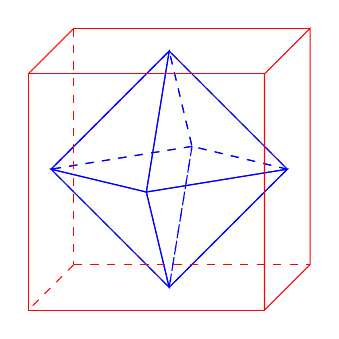
\begin{tikzpicture}[z = -5.5, scale = 1.5]
    \coordinate (O1) at (0, 0, -1);
    \coordinate (O2) at (-1, 0, 0);
    \coordinate (O3) at (0, 0, 1);
    \coordinate (O4) at (1, 0, 0);
    \coordinate (O5) at (0, 1, 0);
    \coordinate (O6) at (0, -1, 0);

    \draw [draw = blue, dashed] (O1) -- (O2) -- (O5) -- cycle;
    \draw [draw = blue, dashed] (O4) -- (O1) -- (O5) -- cycle;
    \draw [draw = blue, dashed] (O1) -- (O2) -- (O6) -- cycle;
    \draw [draw = blue, dashed] (O4) -- (O1) -- (O6) -- cycle;
    \draw [draw = blue] (O2) -- (O3) -- (O5) -- cycle;
    \draw [draw = blue] (O3) -- (O4) -- (O5) -- cycle;
    \draw [draw = blue] (O2) -- (O3) -- (O6) -- cycle;
    \draw [draw = blue] (O3) -- (O4) -- (O6) -- cycle;

    \coordinate (C1) at (-1, -1, -1);
    \coordinate (C2) at (-1, -1, 1);
    \coordinate (C3) at (-1, 1, 1);
    \coordinate (C4) at (-1, 1, -1);
    \coordinate (C5) at (1, -1, -1);
    \coordinate (C6) at (1, -1, 1);
    \coordinate (C7) at (1, 1, 1);
    \coordinate (C8) at (1, 1, -1);

    \draw [draw = red, dashed] (C1) -- (C2);
    \draw [draw = red] (C2) -- (C3);
    \draw [draw = red] (C3) -- (C4);
    \draw [draw = red, dashed] (C4) -- (C1);
    \draw [draw = red] (C5) -- (C6) -- (C7) -- (C8) -- cycle;
    \draw [draw = red, dashed] (C1) -- (C5);
    \draw [draw = red] (C2) -- (C6);
    \draw [draw = red] (C3) -- (C7);
    \draw [draw = red] (C4) -- (C8);
  \end{tikzpicture}
\end{center}
So are icosahedron and dodecahedron. To be dual, it means that they
have exactly the same group of symmetries. So there are only 3 groups
of symmetries for Platonic solids.

We have already seen that if $2||G|$ then $G$ has an element of order
2. Can show that the same thing applies for primes.

\begin{theorem}[Cauchy]\label{thm:Cauchy}
  Let $G$ be a finite group, $p$ be a prime such that $p||G|$, then
  $G$ has an element of order $p$.
\end{theorem}
\begin{proof}
  Let $p||G|$. Consider $ G^p = G\times \cdots \times G $. This is
  the group formed of $p-tuples$ of elements of $G$ with
  coordinate-wise composition. That is,
  \[
    (g_1,\dots,g_p)\cdot (h_1,\dots,h_p)=(g_1h_1,\dots,g_ph_p)
  .\]
  Consider subset $ X \subseteq G $ as
  \[
    X = \left\{ (g_1,\dots,g_p)\in G^p: g_1g_2\cdots g_p = e\right\}
  .\]
  Note that if $g\in G$ with order $p$, then $ (g,g,\dots,g)\in X $.
  Conversely if $ (g,g,\dots,g)\in X, g\neq e $, then $ \ord g=p $ by Lagrange.

  Now take a cyclic group $C_p=\langle a \rangle $ and let $C_p$ act
  on $X$ by \textit{cycling}:
  \[
    a(g_1,\dots,g_p)=(g_2,\dots, g_p,g_1)
  .\]
  This is an action since:
  \begin{enumerate}[(1)]
    \item If $ g_1\cdots g_p=e $, then $
      e=g_1^{-1}eg_1=g_1^{-1}g_1g_2\cdots g_p g_1=g_2\cdots g_pg_1 $.
      Therefore $ a(g_1,\dots,g_p) \in X$. By induction, it is true
      for any power of $a$.
    \item $ e(g_1,\dots,g_p)=g_1,\dots,g_p $ by definition.
    \item $ a^k(g_1,\dots,g_p)=(g_{k+1},\dots,g_k)=a\cdot a\cdot
      \cdots \cdot a(g_1,\dots,g_p) $
  \end{enumerate}
  Since orbit partition $X$, the sum of sizes of distinct orbits must
  be $|X|$. But $|X|=|G|^{p-1}$ because we can choose the first $p-1$
  element arbitrarily and let the last element multiply to $e$. So
  since $ p||G| $, $ p||X| $.

  We have by orbit-stabliser:
  \[
    |\orb(g_1\dots,g_p)||\stab(g_1\dots,g_p)|=|C_p|=p
  .\]
  Hence $|\orb(g_1\dots,g_p)|$ must be of size 1 or $p$, and they sum
  to $|X|=p\cdot Q$ where $Q$ is an integer. Hence,
  \[
    |X|=pQ=\sum_{\orb \text{ of size 1}} 1 + \sum_{\orb\text{ of size }p} p
  .\]
  Clearly $ |\orb(e,e,\dots,e)|=1 $, so there must be at least $p-1$
  other orbits of size 1. But orbits of size 1 must be of the form
  \[
    \{(g,g,\dots,g)\}
  .\]
  So $ \exists g\neq e $ such that $ (g,\dots,g) \in X$, which
  implies that $ \boxed{\ord g = p }$.
\end{proof}
\subsection{Left Multiplication Actions}
\begin{lemma}\label{lma:5.13}
  Let $G$ be a group, $G$ acts on itself by left multiplication. This
  action is faithful and transitive.
\end{lemma}
\begin{proof}
  $ \forall g,x\in G, gx\in G $. $ ex=x $. $ g_1g_2(x)=(g_1g_2)(x) $.
  Hence it is an action. $ g(x)=gx=x \Leftrightarrow g=e $ so it is
  faithful. It is transitive since given $x,y\in G$, we have
  $g=yx^{-1}$ such that $g(x)=y$.
\end{proof}
\begin{definition}
  The left multiplication action of a group on itself is called the
  \textit{left regular action}.
\end{definition}
\begin{theorem}[Cayley]\label{thm:Cayley}
  Every group is isomorphic to a subgroup of a symmetric group.
\end{theorem}
\begin{proof}
  Let $ G \curvearrowright G $ by left regular action. This gives a
  homomorphism $ \rho: G \to \sym G $ with $ \ker \rho=\left\{ e
  \right\} $ since the action is faithful. So by first isomorphism
  theorem, $G/\ker \rho=G \cong \im \rho \subseteq \sym G$.
\end{proof}
\begin{proposition}\label{prop:5.16}
  Let $H\le G$, then $G \curvearrowright G/H$ by left
  multiplication(left coset action) and it is transitive.
\end{proposition}
\begin{proof}
  $ g(g_1H)=gg_1H\in G/H $. $ e(g_1H)=g_1H $. $
  g_1(g_2(g_3H))=(g_1g_2)g_3H $. So it is an action. Given two cosets
  $ g_1H,g_2H $, have $ (g_1g_2^{-1})(g_2H)=g_1H $, so it is transitive.
\end{proof}
\begin{remark}
  This is the left regular action if $H$ is trivial. This induces
  actions of $G$ on its quotient groups $G/N$.
\end{remark}
\subsection{Conjugation Action}
\subsubsection{Basics}
\begin{definition}
  Given $g,h\in G$, the element $hgh^{-1}\in G$ is the
  \textit{conjugate} of $g$ by $h$.
\end{definition}
We should think of conjugate elements as doing the same thing from
different points of view. This will become particularly clear when we
look at M\"{o}bius maps and matrices later.
\begin{example}
  Consider $D_{10}$ and consider the conjugate $s$ and $rsr^{-1}$
  where $s$ is reflection through $v_1$ and $r$ is rotation by
  $2\pi/5 $. It is clear that $rsr^{-1}$ is the reflection through $v_2$.
\end{example}
\begin{example}\footnote{You can expect conjugate elements to have
  similar properties. e.g., same order.}
  Consider matrix groups such as $ \mathrm{GL}_2(\mathbb{R}) $ where
  a conjugate matrix represents the same transformation, but wrt a
  different basis. Will talk about this later.
\end{example}
\begin{proposition}\label{prop:5.18}
  A group $G$ acts on itself by conjugation.
\end{proposition}
\begin{proof}
  $g(x)=gxg^{-1}\in G$. $exe^{-1}=x$. $
  g(h(x))=g(hxh^{-1})=ghxh^{-1}g^{-1}=(gh)x(gh)^{-1}=(gh)(x) $. Hence
  it is an action.
\end{proof}
The kernel, orbits and stablisers have special names:
\begin{definition}
  The kernel of the conjugation action $ G \curvearrowright G $ is
  called \textit{center} $ Z(G) $ of $G$:
  \[
    Z(G)=\left\{ g\in G: ghg^{-1}=h, \forall h \right\}
    \Longleftrightarrow Z(G)=\left\{ g\in G: gh=hg \right\}
  .\]
  That is, the elements that commute with every other element.

  An orbit of this action is called \textit{conjugacy class}:
  \[
    \mathbb{C}l(h)=\left\{ ghg^{-1}:g\in G \right\} \text{ or } \mathbb{C}l_G(h)
  .\]

  Stablisers are called \textit{centralisers}
  \[
    C_G(h)=\left\{ g\in G:ghg^{-1}=h \right\}
  .\]
  That is, elements that commute $h$.
\end{definition}
\begin{proposition}
  $\displaystyle Z(G)=\bigcap_{h\in G}C_G(h)$.
\end{proposition}
\begin{proof}
  Let $g\in Z(G)$. Then $\forall h\in G, ghg^{-1}=h \Rightarrow
  \forall h\in G, g\in C_G(h) \Rightarrow Z(G)\subseteq \bigcap
  C_G(h)$. Conversely let $ g\in \bigcap C_G(h) $, then $ \forall h,
  ghg^{-1}=h \Rightarrow g\in Z(G) \Rightarrow \bigcap C_G(h)
  \subseteq Z(G) $. Hence $ Z(G)=\bigcap_{h\in G}C_G(h) $.
\end{proof}
\begin{definition}
  If $H\le G$ and $g\in G$, the \textit{conjugate of $H$ by $g$} is
  \[
    gHg^{-1}=\left\{ ghg^{-1}:h\in H \right\}
  .\]
\end{definition}
\begin{proposition}\label{prop:5.21}
  Let $H\le G$, $g\in G$. Then $gHg^{-1}$ is also a subgroup of $G$.
\end{proposition}
\begin{proof}
  $e\in gHg^{-1}$. Let $gh_1g^{-1},gh_2g^{-1}\in gHg^{-1}$. Then $
  gh_1g^{-1}(gh_2g^{-1})^{-1}=gh_1g^{-1}gh_2^{-1}g^{-1}gh_1h_2^{-1}g^{-1}\in
  gHg^{-1} $.
\end{proof}
\begin{proposition}
  $ gHg^{-1} \cong H $.
\end{proposition}
\begin{proof}
  Let $ \varphi: H \to gHg^{-1} $ by $ \varphi(h)=ghg^{-1} $. Indeed,
  it is a homomorphism. It is clearly a bijection so it is an isomorphism.
\end{proof}
\begin{proposition}\label{prop:5.22}
  A group $G$ acts by conjugation on the set of its subgroups. The
  singleton orbits are the normal subgroups.
\end{proposition}
\begin{proof}
  Let $H\le G, g\in G$. $ gHg^{-1}\le G $ so it is closed under
  conjugation. Obviously $ eHe^{-1}=H $ and $
  g_1(g_2(H))=g_1(g_2Hg_2^{-1})=g_1g_2H(g_1g_2)^{-1}=(g_1g_2)(H) $.
  Therefore it is an action. Let $N \le G$ that has a singleton
  orbit. Since $eNe^{-1}=N$, $ \orb(N) $ must be $N$ itself. By
  definition of normal subgroups, $ N \ltrigeq G $.
\end{proof}
\begin{remark}
  This gives another view of point of normal subgroups: they are
  invariant under conjugation.
\end{remark}
\begin{proposition}\label{prop:5.23}
  Normal subgroups are those subgroups that are union of conjugacy classes.
\end{proposition}
\begin{proof}
  Let $ N \ltrigeq G $. Then if $ h\in N $, then $ghg^{-1}\in N$ for
  all $g\in G$, so $ \mathbb{C}l(h) \subseteq N $. Therefore,
  \[
    N=\bigcup_{h\in N} \mathbb{C}l(h)
  .\]
  Conversely, if $H$ is a subgroup that is a union of conjugacy
  classes, then $ \forall g\in G, h\in H, ghg^{-1}\in H
  \Leftrightarrow H \ltrigeq G $.
\end{proof}
\begin{example}
  Consider $ A_3=\left\{ e,(123),(132) \right\} $. In fact
  \[
    A_3 = \{e\}\sqcup \{(123),(132)\}
  .\]
\end{example}
\begin{remark}
  Note that $ (123),(132) $ are conjugate in $S_3$, but not in $A_3$.
\end{remark}
\subsubsection{Conjugation in $S_n$}
\begin{lemma}\label{lma:5.24}
  Given a $k$-cycle, $(a_1\ a_2\ \cdots\ a_k)$ and $ \sigma\in S_n $, we have
  \[
    \sigma(a_1\ \cdots
    \ a_k)\sigma^{-1}=(\sigma(a_1)\ \sigma(a_2)\ \cdots\ \sigma(a_k))
  .\]
\end{lemma}
\begin{proof}
  Let's look at where the elements are sent.
  \[
    \begin{aligned}
      &\sigma(a_i) \mapsto a_i \mapsto a_{i+1} \mapsto \sigma(a_{i+1}),\\
      &a \mapsto \sigma^{-1}(a) \mapsto \sigma^{-1}(a) \mapsto
      a,\quad \text{for $a\notin \left\{ \sigma(a_1),\dots,
      \sigma(a_k) \right\}$.}
    \end{aligned}
  \]
  RHS does the same thing as LHS, so $ \sigma(a_1\ \cdots
  \ a_k)\sigma^{-1}=(\sigma(a_1)\ \sigma(a_2)\ \cdots\ \sigma(a_k)) $.
\end{proof}
\begin{proposition}\label{prop:5.25}
  Two elements of $S_n$ are conjugate (in $S_n$, i.e.,
  $\tau=\rho\sigma\rho^{-1}$ for some $\rho \in S_n$), if and only if
  they have \underline{the same cycle type}.
\end{proposition}
\begin{proof}
  Take $ \sigma, \tau\in S_n $ such that $ \sigma, \tau $ are
  conjugate. Write $ \sigma $ in disjoint cycles:
  \[
    \sigma=\sigma_1\sigma_2\cdots \sigma_m
  ,\]
  then if $ \tau=\rho\sigma\rho^{-1} $
  \[
    \begin{aligned}
      \tau&=\rho\sigma_1\sigma_2\cdots \sigma_m\rho^{-1}\\
      &= \rho\sigma_1\rho^{-1}\rho\sigma_2\rho^{-1}\cdots \rho\sigma_m\rho^{-1}.
    \end{aligned}
  \]
  By \ref{lma:5.24}, each $ \rho\sigma\rho^{-1} $ is a cycle of the
  same length as $\sigma_i$, and the $ \rho\sigma_i\rho^{-1} $ are
  disjoint, since $\rho$ is a bijction. Hence $ \sigma,\tau $ have
  the same cycle type.

  Conversely if $\sigma,\tau$ have the same cycle types, then can write
  \[
    \begin{aligned}
      &\sigma= (a_1\ \cdots\ a_{k_1})(a_{k_1+1}\ \cdots\ a_{k_2})\cdots\\
      &\tau = (b_1\ \cdots\ b_{k_1})(b_{k_1+1}\ \cdots\ b_{k_2})\cdots
    \end{aligned}
  \]
  in disjoint cycle notation, including singletons, so that all of
  $\{1,\dots,n\}$ appear in the notation.

  Construct $ \rho $ as $ \rho(a_i)=b_i, \forall i$, which is indeed
  a permutation. Then $ \rho\sigma\rho^{-1}=\tau $.
\end{proof}
\begin{example}[Conjugate classes of $S_4$]
  \begin{center}
    \begin{tabular}{c|c|c|c|c}
      Cycle Type & Example Element & Size of $\mathbb{C}l$ & Size of
      $C_{S_4}$ & Sign \\
      \hline
      & & & \redcomment{$ |S_4|/|\mathbb{C}l| $} & \\
      1,1,1,1 & $e$ & 1 & $24/1=24$ &1 \\
      2,1,1 & $(1\ 2)$ & 6 & 4 &-1 \\
      2,2 & $(1\ 2)(3\ 4)$ & 3 & 8 &1 \\
      3,1 & $(1\ 2\ 3)$ & 8 & 3 &1 \\
      4 & $(1\ 2\ 3\ 4)$ & 6 & 4 &-1 \\
    \end{tabular}
  \end{center}
  From this, we can work out the normal subgroups of $S_4$:
  \begin{itemize}
    \item Must contain $e$,
    \item Must be a union of conjugacy classes,
    \item Must have order dividing $|G|$.
  \end{itemize}
  Possibilities: look through divisors of $|G|$: 1,2,3,4,6,8,12,24.
  \begin{enumerate}[align=left, label=\textit{order} \arabic*]
    \item $ \left\{ e \right\} $.
    \item Not possible.
    \item Not possible.
    \item $ \left\{ e,(12)(34),(13)(24),(14)(23) \right\} \cong C_2
      \times C_2=:V_4 $, Klein 4 group.
    \item[\textit{order} 6] Not possible.
    \item[\textit{order} 8] Not possible.
    \item[\textit{order} 12] $ \{e,(12)(34),(13)(24),(14)(23), (123),
      (132),(124),(142),(134),(143),(234),(243)\}$, which is exactly $A_4$.
    \item[\textit{order} 24] $S_4$.
  \end{enumerate}
  So all possible quotients of $S_4$ are:
  \begin{itemize}
    \item $ S_4/\{e\}\cong S_4 $.
    \item $ S_4/V_4 = \left\{
      V_4,(12)V_4,(13)V_4,(23)V_4,(123)V_4,(132)V_4 \right\} \cong S_3 $.
    \item $ S_4/A_4 \cong C_2 $.
    \item $ S_4/S_4 \cong \left\{ e \right\} $.
  \end{itemize}
  Can repeat this with $S_5$.
\end{example}
\subsubsection{Conjugation in $A_n$}

Note that
\[
  \mathbb{C}l_{A_n}(\sigma)=\left\{ \tau \sigma\tau^{-1}:\tau\in A_n
  \right\} \subseteq \mathbb{C}l_{S_n}(\sigma)
.\]
But elements that are conjugate in $S_n$ may not be conjugate in
$A_n$. e.g., $ (23)(123)(23)=(132) $ in $S_3$ but $ (23)\notin A_3 $
so there is no other elements forming the conjugation.

However, in $S_5, (23)(45)(123)(45)(23)=(132)$, so $ (123),(132) $
are conjugate in $A_5$.

Some conjugacy classes may split into smaller conjugacy classes in
$A_n$. But how?

By orbit-stabliser, $
|S_n|=|\mathbb{C}l_{S_n}(\sigma)||C_{S_n}(\sigma)| $ and $
|A_n|=|\mathbb{C}l_{A_n}(\sigma)||C_{A_n}(\sigma)| $. But $
|S_n|=2|A_n| $ and $ |\mathbb{C}l_{A_n}(\sigma)|\le
|\mathbb{C}l_{S_n}(\sigma)| $, so either
\[
  \mathbb{C}l_{A_n}(\sigma)=\mathbb{C}l_{S_n}(\sigma) \text{ and }
  |C_{A_n}(\sigma)|=\frac{1}{2}|C_{S_n}(\sigma)|
\]
or
\[
  |\mathbb{C}l_{A_n}(\sigma)|=\frac{1}{2}
  |\mathbb{C}l_{S_n}(\sigma)|\text{ and } C_{A_n}(\sigma)=C_{S_n}(\sigma)
.\]
\begin{definition}
  When $|\mathbb{C}l_{A_n}(\sigma)|=\frac{1}{2}
  |\mathbb{C}l_{S_n}(\sigma)|$, we say that the conjugacy class of $
  \sigma $ \textit{splits} in $A_n$.
\end{definition}
To see when it happens, we have the following proposition:
\begin{proposition}\label{prop:5.28}
  The ccl of $ \sigma $ in $A_n$ splits in $A_n$ if and only if no
  odd permutations commute with $\sigma$.
\end{proposition}
\begin{proof}
  Note that
  \[
    |\mathbb{C}l_{A_n}(\sigma)|=\frac{1}{2}
    |\mathbb{C}l_{S_n}(\sigma)| \Longleftrightarrow
    C_{A_n}(\sigma)=C_{S_n}(\sigma)
  ,\]
  so $ C_{A_n}(\sigma)=A_n \cap C_{S_n}(\sigma) $. However, $ A_n
  \cap C_{S_n}(\sigma) =C_{S_n}(\sigma) $ if and only if
  $C_{S_n}(\sigma)$ has no odd elements. i.e., no odd permutations
  commute with $ \sigma $.
\end{proof}
\begin{example}[Conjugate classes of $A_4$]
  \begin{center}
    \begin{tabular}{c|c|c|c|c}
      Cycle Type & Example Element & Odd element in $C_{S_4}$? &
      $|\mathbb{C}l_{S_4}|$ & $|\mathbb{C}l_{A_4}|$ \\
      \hline
      1,1,1,1 & $e$ & yes, eg. $(1\ 2)$ & 1 & 1\\
      2,2 & $(1\ 2)(3\ 4)$ & yes eg. $(1\ 2)$ & 3 & 3\\
      3,1 & $(1\ 2\ 3)$ & no\footnote{Since $ |C_{S_4}|=3 $ and
        clearly contains $(123)$ itself, so $ C_{S_4}=\langle (123)
      \rangle $} & 8 & 4 and 4\\
    \end{tabular}
  \end{center}
\end{example}
\begin{example}[Conjugate classes of $A_5$]
  \begin{center}
    \begin{tabular}{c|c|c|c|c}
      Cycle Type & Example Element & Odd element in $C_{S_5}$? &
      $|\mathbb{C}l_{S_5}|$ & $|\mathbb{C}l_{A_5}|$ \\
      \hline
      1,1,1,1,1 & $e$ & yes, eg. $(1\ 2)$ & 1 & 1\\
      2,2,1 & $(1\ 2)(3\ 4)$ & yes eg. $(1\ 2)$ & 15 & 15\\
      3,1,1 & $(1\ 2\ 3)$ & yes eg. $(4\ 5)$ & 20 & 20\\
      5 & $(1\ 2\ 3\ 4\ 5)$ & no, see lemma & 24 & 12 and 12\\
    \end{tabular}
  \end{center}
  \begin{lemma}\label{lma:5.31}
    $ C_{S_5}(12345)=\langle (12345) \rangle $.
  \end{lemma}
  \begin{proof}
    Note that $ |\mathbb{C}l(12345)|=5!/5=24 $. By orbit-stabliser, $
    |C_{S_5}(12345)|=5 $, and it is clear that
    $C_{S_5}(12345)=\langle (12345) \rangle$.
  \end{proof}
\end{example}
\begin{theorem}\label{thm:5.32}
  $A_5$ is a simple group.
\end{theorem}
\begin{proof}
  Normal subgroups must be unions of conjugacy classes, must contain
  $e$ and the order must divide $|A_5|=60$. The sizes of conjugacy
  classes in $A_5$ are $1,15,20,12,12$. The only ways of adding 1
  plus some of the sizes to get a number dividing 60 are $ 1 $ and $
  1+15+20+12+12=60 $. Hence the normal subgroups of $A_5$ are $\{e\}$
  and $A_5$. Therefore it is simple.
\end{proof}
\begin{remark}
  All $A_n, n\ge 5$ are simple.
\end{remark}

\subsection{The \mobius Group Revisited}
\subsubsection{Basic Properties}
We now have the tools to study the actions of the \mobius group $ \mathcal{M} $.
\begin{remark}
  The definition of \mobius maps defines an action $ \mathcal{M}
  \curvearrowright \hat{\mathbb{C}} $.
\end{remark}
\begin{proposition}\label{prop:6.1}
  The action $ \mathcal{M} \curvearrowright \hat{\mathbb{C}} $ is
  faithful, and so $ \mathcal{M}\le \sym(\hat{\mathbb{C}}) $.
\end{proposition}
\begin{proof}
  Consider $ \rho: \mathcal{M} \to \sym(\hat{\mathbb{C}}) $ defined
  by $ \rho(f)(z)=f(z) $. Can verify that $ \rho $ is injective and
  the action is faithful.
\end{proof}
\begin{definition}
  A \textit{fixed point} of a \mobius map $f$ is a point $z\in
  \hat{\mathbb{C}}$ such that $ f(z)=z $.
\end{definition}
\begin{theorem}\label{thm:6.3}
  A \mobius map with $\ge 3$ fixed points is the identity.
\end{theorem}
\begin{proof}
  Let $ f=az+b/cz+d $ have $\ge 3$ fixed points. Then if $\infty$ is
  not a fixed point,
  \[
    \frac{az+b}{cz+d}=z \Longleftrightarrow cz^2+(d-a)z-b=0
  \]
  has $\ge 3$ roots. But a quadratic equation has $\le 2$ roots, so
  $c=b=0$ and $d=a$. i.e., $f$ is the identity.
  If $\infty$ is a fixed point, so $ a/c=\infty \Leftrightarrow c=0 $. So
  \[
    \frac{az+b}{d}=z \Longleftrightarrow (a-d)z+b=0
  \]
  has $\ge 2$ roots, and similarly $f$ is the identity.
\end{proof}
\begin{corollary}\label{col:6.4}
  If two \mobius maps coincide on 3 distinct points in $
  \hat{\mathbb{C}} $ then they are equal.\footnote{Knowing what a
    \mobius map does on 3 distinct points in $ \hat{\mathbb{C}} $
  \textit{uniquely} determines it.}
\end{corollary}
\begin{proof}
  Apply theorem \ref{thm:6.3} on $g^{-1}f$.
\end{proof}
\begin{theorem}\label{thm:6.5}
  There is a unique \mobius map sending any 3 distinct points of $
  \hat{\mathbb{C}} $ to any 3 distinct points of $ \hat{\mathbb{C}}
  $. i.e., given $ z_1,z_2,z_3, w_1,w_2,w_3\in \hat{\mathbb{C}} $
  distinct, $ \exists ! f, f(z_i)=w_i $ for $i=1,2,3$.
\end{theorem}
\begin{proof}
  Suppose first that $w_1=0,w_2=1,w_3 = \infty $. Then we can take
  \[
    f(z)=\frac{(z_2-z_3)(z-z_1)}{(z_2-z_1)(z-z_3)}.
  \]
  Particularly, if $z_1=\infty$, take $ f(z)=\frac{z_2-z_3}{z-z_3} $;
  if $z_2=\infty$, take $ f(z)=\frac{z-z_1}{z-z_3} $; if
  $z_3=\infty$, take $ f(z)=\frac{z-z_1}{z_2-z_1} $. Thus we have
  found a function $ f_1: (z_1,z_2,z_3) \mapsto (0,1, \infty ) $ and
  $ f_2:(w_1,w_2,w_3)\mapsto (0,1,\infty ) $. Now consider
  \[
    f = f_2^{-1}\circ f_1: (z_1,z_2,z_3)\mapsto (w_1,w_2,w_3),
  \]
  as required.

  Uniqueness follows trivially from corollary \ref{col:6.4}.
\end{proof}
From example sheet 2 we see that:
\begin{proposition}\label{prop:egsheet2}
  A conjugate $ hfh^{-1} $ of a \mobius map satisfies:
  \begin{enumerate}
    \item $ \ord(hfh^{-1})=\ord(f) $;
    \item $f$ fixes $z \Leftrightarrow hfh^{-1}$ fixes $h(z)$.
  \end{enumerate}
  In particular, the number of fixed point is invariant.
\end{proposition}
The following theorem is a partial converse to this observation:
\begin{theorem}\label{thm:6.6}
  Every non-identity $f\in \mathcal{M}$ has either 1 or 2 fixed
  points. If $f$ has 1 fixed point, then it is conjugate to $ z
  \mapsto z+1 $. If $f$ has 2 fixed points, then it is conjugate to a
  map of the form $ z \mapsto az, a\in \hat{\mathbb{C}}\setminus \{0\} $.
\end{theorem}
\begin{proof}
  It suffices to show that $f$ cannot have 0 fixed point.
  If $ f(z)=\frac{az+b}{cz+d} $, consider the quadratic
  \[
    cz^2+(d-a)z-b \Longleftrightarrow f(z)=z,
  \]
  it has at least one solution since $ \Delta\ge 0 $, so $f$ has at
  least one fixed point.

  If $f$ has 1 fixed point $z_0$, choose $z_1\in \mathbb{C}$ not
  fixed by $f$. Then $ z_1,f(z_1),z_0 $ are all distinct. Hence $
  \exists g:(z_1,f(z_1),z_0)\mapsto (0,1,\infty) $. Consider $
  gfg^{-1}: 0 \mapsto 1, \infty \mapsto \infty $. Claim that
  $gfg^{-1}$ is of the form $ az+1,a\in \mathbb{C} $. Indeed, any map
  of the form $az+1$ has the two properties. The other direction
  follows by direct substitution in the general form
  $\frac{az+b}{cz+d}$. If $a\neq 1$, $gfg^{-1}$ has $
  \frac{1}{1-a}\neq \infty  $ as a fixed point, \# since we only
  supposed 1 fixed point. Hence $f$ is conjugate to $z+1$.

  If $f$ has 2 fixed points $z_0,z_1$, consider $ g:(z_0,z_1) \mapsto
  (0,\infty ) $. We have $ gfg^{-1}:(0,\infty ) \mapsto (0,\infty )
  $, so that $gfg^{-1}$ fixes $0$ and $\infty$. Claim that $g$ is of
  the form $az$. Indeed, take $ a=gfg^{-1} $, then substitution in
  the general form gives the answer.
\end{proof}
We can use this to work out $f^n$ for any $ f\in \mathcal{M} $.
Indeed, if $f$ fixes one point, then $gf^ng^{-1}=(gfg^{-1})^n=z+n$.
Similarly if $f$ fixes 2 points then $ gf^ng^{-1}=a^n z $.
\subsubsection{Circles and Lines}
Equation of a circle with centre $b\in \mathbb{C}$ and radius $r>0$ is
\[
  |z-b|=r \Longleftrightarrow z \bar{z}- \bar{b}z-b \bar{z}+ b
  \bar{b}-r^2=0.\tag{$*$}
\]
Equation of a line in $\mathbb{C}$:
\[
  a \Re (z)+b \Im (z)=c(a,b,c\in \mathbb{R}) \Longleftrightarrow
  \overline{\frac{a+ib}{2}}z+\frac{a+ib}{2}\bar{z}-c=0.\tag{$ \dagger $}
\]
For a line in $ \hat{\mathbb{C}} $ we also consider $ \infty  $ is
always on the line, this can be visualised by using stereographic
projection. These lines are also circles through the north pole.

Both $ (*) $ and $(\dagger)$ have the form in the next definition:
\begin{definition}
  A \textit{circle} in $ \hat{\mathbb{C}} $ is the set of points
  satisfying the equation
  \[
    Az \bar{z}+ \overline{B}z+B \bar{z}+C=0,
  \]
  with $ A,C,\in \mathbb{R}, B\in \mathbb{C}, |B|^2>AC $. We consider
  $ \infty  $ to be a solution if and only if $A=0$.
\end{definition}

\begin{exercise}
  The set of points satisfying such an equation is always either a
  circle in $\mathbb{C}$ or a line with $ \infty $.
\end{exercise}

We call all of these object circles in $ \hat{\mathbb{C}} $ by convention.
\begin{remark}
  We shouldn't think of $\infty$ as a "special" point.
\end{remark}

\begin{theorem}\label{thm:6.8}
  \mobius maps send circles to circles in $ \hat{\mathbb{C}} $.
\end{theorem}
\begin{proof}
  By proposition \ref{prop:decomp_mobius}, it suffices to check $
  f_1=az,f_2=z+b,f_3=\frac{1}{z} $ have this property. Write
  $S(A,B,C)$ for the circle
  \[
    Az \bar{z}+ \overline{B}z+B \bar{z}+C=0. %\tag{$\clubsuit $}
  \]
  We can check that
  \begin{align*}
    f_1&: S(A,B,C)\mapsto S\left(
    \frac{A}{\bar{a}a},\frac{B}{\bar{a}},C \right),\\
    f_2&: S(A,B,C)\mapsto S(A,B-Ab,C+Ab \bar{b}-B \bar{b}- \overline{B}b),\\
    f_3&: S(A,B,C) \mapsto S(C,\overline{B},A).
  \end{align*}
\end{proof}
\begin{remark}
  A circle is determined by 3 points on it, and a \mobius map is
  determined by where it sends 3 points. In practice, it is easy to
  find a \mobius map sending a given circle to another given circle.
\end{remark}
\begin{example}
  Want a \mobius map $f$ that sends the unit circle to the circle $
  \mathbb{R} \cup \{\infty\} $, the real line. Pick $ \{-1,i,1\} $ on
  the unit circle and pick $ \{-1,0,1\} $ on $ \mathbb{R} \cup
  \{\infty \} $. We want $-1,1$ fixed and $ i \mapsto 0 $. For example
  \[
    f(z)=\frac{z-i}{1-iz}.
  \]
  There are many choices.
\end{example}
\subsubsection{Cross-Ratios}
Recall that given $z_1,z_2,z_3 \in \hat{\mathbb{C}}$ distinct, $
\exists !f\in \mathcal{M}, f(z_1)=0, f(z_2)=1,f(z_3)=\infty  $.
\begin{definition}
  If $z_1,z_2,z_3,z_4 \in \hat{\mathbb{C}}$ distinct, then the
  \textit{cross ratio} $ [z_1,z_2,z_3,z_4] $ is defined to be
  $f(z_4)$, where $f$ is the function above.

  In particular, $ [0,1,\infty,w]=w $.
\end{definition}
We have the following formula:
\begin{proposition}
  \[
    [z_1,z_2,z_3,z_4] = \frac{(z_2-z_3)(z_4-z_1)}{(z_2-z_1)(z_4-z_3)}
  \]
  with special cases interpreted accordingly.
\end{proposition}
\begin{proof}
  Refer to theorem \ref{thm:6.5}.
\end{proof}
\begin{proposition}\label{prop:6.10}
  Double transpositions of the $z_i$ fix the cross-ratio.
\end{proposition}
\begin{proof}
  By inspection.
\end{proof}
\begin{theorem}\label{thm:6.11}
  \mobius maps preserve cross-ratios. i.e., $ \forall g\in
  \mathcal{M}, \forall z_1,z_2,z_3,z_4\in \hat{\mathbb{C}} $ distinct,
  \[
    [g(z_1),g(z_2),g(z_3),g(z_4)]=[z_1,z_2,z_3,z_4].
  \]
\end{theorem}
\begin{proof}
  Let $f$ be the unique \mobius map $ (z_1,z_2,z_3)\mapsto
  (0,1,\infty ) $, so that
  \[
    f(z_4)=[z_1,z_2,z_3,z_4].
  \]
  Consider $ fg^{-1}: g(z_1)\mapsto 0,g(z_2)\mapsto 1,g(z_3)\mapsto
  \infty  $. Hence $fg^{-1}$ is the unique map that does this and we have
  \[
    [g(z_1),g(z_2),g(z_3),g(z_4)] = fg^{-1}(g(z_4))=f(z_4)=[z_1,z_2,z_3,z_4],
  \]
  as required.
\end{proof}
\begin{corollary}\label{col:6.12}
  Four distinct points $z_1,z_2,z_3,z_4\in \hat{\mathbb{C}}$ lie on a
  circle if and only if $[z_1,z_2,z_3,z_4]\in \mathbb{R}$.
\end{corollary}
\begin{proof}
  Let $f\in \mathcal{M}: (z_1,z_2,z_3)\mapsto (0,1,\infty )$, so that
  $ f(z_4)=[z_1,z_2,z_3,z_4] $. The circle $C$ through $z_1,z_2,z_3$
  is sent to the circle through $0,1,\infty$, i.e., the real axis.
  Hence $z_4$ lies on the circle if and only if $f(z_4)$ is on the
  real line, i.e., $[z_1,z_2,z_3,z_4]\in \mathbb{R} \cup \{\infty\}
  \Leftrightarrow [z_1,z_2,z_3,z_4]\in \mathbb{R}$ since $f(z_3)=\infty$.
\end{proof}
\subsection{Matrix Groups}
\subsubsection{Some Matrix Groups}
Denote $ \mathcal{M}_{n\times n}(\mathbb{F}) $ for the set of $ n
\times n $ matrices over the field $\mathbb{F}$, typically
$\mathbb{R},\mathbb{C}$.

\begin{definition}
  The \textit{general linear group} over $\mathbb{F}$ is defined by
  \[
    \GL_n(\mathbb{F})=\left\{ A\in \mathcal{M}_{n\times
    n}(\mathbb{F}):A \text{ is invertible} \right\}.
  \]
\end{definition}
\begin{proposition}
  \begin{itemize}
    \item $ \GL_n(\mathbb{F}) \to \mathbb{F}^*:=\mathbb{F} \setminus
      \{0\} $ is a surjective homomorphism.
  \end{itemize}
\end{proposition}
\begin{definition}
  The \textit{special linear group} $ \SL_n(\mathbb{F}) \le
  \GL_n(\mathbb{F}) $ is defined by $ \SL_n(\mathbb{F}) = \ker \det $.
\end{definition}
\begin{definition}
  The \textit{orthogonal group} $ \Or_n=\Or_n(\mathbb{R})=\{A\in
  \GL_n(\mathbb{R}): A^\top A=I\} $.
\end{definition}
\begin{proposition}\label{prop:7.4}
  $ \det : \Or_n\to \left\{ \pm 1 \right\} $ is a surjective homomorphism.
\end{proposition}
\begin{proof}
  If $A\in \Or_n$ then $A^\top A=I$, so
  \[
    \det (A)^2=\det A^\top \det A = \det (A^\top A)=\det I=1
    \Longleftrightarrow \det A=\pm 1.
  \]
  It is surjective since $ \det I=1, \det \tilde{I}=-1 $, where
  \[
    \tilde{I}=
    \begin{pmatrix}
      -1&\cdots &\cdots &0\\
      \vdots &1& \cdots &\vdots \\
      \vdots &\vdots &\ddots &\vdots \\
      0&\cdots&\cdots &1
    \end{pmatrix}.
  \]
  $ \det  $ is indeed a homomorphism as in $ \GL_n(\mathbb{R}) $.
\end{proof}
\begin{definition}
  The \textit{special orthogonal group} $ \SO_n=\SO_n(\mathbb{R}) =
  \ker \det $. i.e.,
  \[
    \SO_n=\{A\in \Or_n:\det A=1\}.
  \]
\end{definition}
\begin{proposition}\label{prop:7.6}
  The function $ \varphi:\SL_2(\mathbb{C})\to \mathcal{M} $ defined by
  \[
    \begin{pmatrix}
      a&b\\
      c&d
    \end{pmatrix} \mapsto \frac{az+b}{cz+d}
  \]
  is a surjective homomorphism with kernel $ \{\pm I\} $.
\end{proposition}
\begin{proof}
  The fact that $ \varphi $ is a homomorphism follows by some
  algebras. If $ \frac{az+b}{cz+d} $ is a \mobius map, check
  \[
    D^2=\det
    \begin{pmatrix}
      a&b\\
      c&d
    \end{pmatrix} \Longrightarrow \det
    \begin{pmatrix}
      a/D&b/D\\
      c/D&d/D
    \end{pmatrix}=D^{-2}D^2=1.
  \]
  The transformed matrix represents the same \mobius map. It follows
  that $ \varphi $ is surjective.

  For kernel, note that
  \[
    \varphi
    \begin{pmatrix}
      a&b\\
      c&d
    \end{pmatrix}=\operatorname{id}\in \mathcal{M}
    \Longleftrightarrow \forall z\in
    \hat{\mathbb{C}},\frac{az+b}{cz+d}=z \Longleftrightarrow
    c=b=0,a=d \Longleftrightarrow
    \begin{pmatrix}
      a&b\\
      c&d
    \end{pmatrix}=
    \begin{pmatrix}
      a&0\\
      0&a
    \end{pmatrix}.
  \]
  Since $ A\in \SL_2(\mathbb{C}) $, $a=\pm 1$ and thus $ \ker
  \varphi=\{\pm I\} $, as claimed.
\end{proof}
\begin{corollary}\label{col:7.7}
  $ \mathcal{M} \cong \SL_2(\mathbb{C})/\{\pm I\} $.
\end{corollary}
\begin{proof}
  By 1st isomorphism theorem.
\end{proof}
\begin{remark}
  The quotient $\SL_2(\mathbb{C})/\{\pm I\}$ is known as the
  \textit{projective special linear group}, denoted by $ \PSL_2(\mathbb{C}) $.
\end{remark}
\subsubsection{Actions of Matrix Groups}
All of the groups defined above act on the corresponding vector space. i.e.,
\[
  \GL_n(\mathbb{F}),\SL_n(\mathbb{F}) \curvearrowright \mathbb{F}^n;
  \Or_n,\SO_n \curvearrowright \mathbb{R}^n
\]
via $ A(\mathbf{x})=A\mathbf{x} $.

\begin{example}
  Let $ G\le \GL_2(\mathbb{R})\curvearrowright \mathbb{R}^2 $.
  Consider its orbits.

  $ \{\mathbf{0}\} $ is always a singleton orbit. If $
  G=\GL_2(\mathbb{R}) $, then $G$ acts transitively on $
  \mathbb{R}^{2}\setminus\{0\} $ since can complete any $
  \mathbf{v}\neq \mathbf{0} $ to a basis and have an invertible
  change of basis matrix sending any basis to any other basis. Hence
  we have 2 orbits, $ \mathbb{R}^{2}\setminus\{0\} $ and $ \{0\} $.
\end{example}
\begin{example}
  Let $ G = \left\{
    \begin{pmatrix} a&b\\0&d
  \end{pmatrix}\in \GL_2(\mathbb{R}) \right\}=\left\{
    \begin{pmatrix} a&b\\0&d
  \end{pmatrix}:a,d\neq 0 \right\} $. Note that
  \begin{align*}
    \orb
    \begin{pmatrix}
      0\\0
    \end{pmatrix}&=\left\{
      \begin{pmatrix}
        0\\0
    \end{pmatrix} \right\},\\
    \orb
    \begin{pmatrix}
      1\\0
    \end{pmatrix}&=\left\{
      \begin{pmatrix} a&b\\0&d
      \end{pmatrix}
      \begin{pmatrix}
        1\\0
      \end{pmatrix}:
      \begin{pmatrix} a&b\\0&d
    \end{pmatrix}\in G \right\} = \left\{
      \begin{pmatrix}
        a\\0
    \end{pmatrix}:a\neq 0 \right\},\\
    \orb
    \begin{pmatrix}
      0\\1
    \end{pmatrix}&=\left\{
      \begin{pmatrix} a&b\\0&d
      \end{pmatrix}
      \begin{pmatrix}
        0\\1
      \end{pmatrix}:
      \begin{pmatrix} a&b\\0&d
    \end{pmatrix}\in G \right\} = \left\{
      \begin{pmatrix}
        b\\d
    \end{pmatrix}:d\neq 0 \right\}.
  \end{align*}
  We can see that they partition $ \mathbb{R}^{2} $.
\end{example}
See example sheet 4 for some other examples.

\subsubsection{Change of Basis}
We now interpret the conjugation of $ \GL_n(\mathbb{F}) $ on $
\mathcal{M}_{n\times n}(\mathbb{F}) $ using change of basis.

Recall that $ \alpha: \mathbb{F}^n \to \mathbb{F}^n $ is a linear
map, we can interpret $\alpha$ with $A$ wrt a basis $
\{\mathbf{e}_1,\dots,\mathbf{e}_n\} $ of $ \mathbb{F}^n $. If we have
a different basis $ \{\mathbf{f}_1,\dots,\mathbf{f}_n\} $, $\alpha$
will be interpreted wrt this basis by $ P^{-1}AP $ where $P$ is the
change of basis matrix. This is an example of conjugation.
\begin{proposition}\label{prop:7.9}
  $ \GL_n(\mathbb{F}) \curvearrowright \mathcal{M}_{n\times
  n}(\mathbb{F}) $ by conjugation.
  \[
    \orb(A)=\left\{ M\in \mathcal{M}_{n\times n}(\mathbb{F}): M
    \text{ represents the same linear map wrt different bases} \right\}.
  \]
\end{proposition}
\begin{proof}
  It is easy to check that conjugation is indeed an action. To see
  the orbits, note that $ A,B $ are on the same orbit if and only if
  $ \exists P\in \GL_n(\mathbb{F}), A = PBP^{-1} \Leftrightarrow B=P^{-1}AP $.
\end{proof}
\begin{example}
  Recall from Vectors and Matrices that every matrix in $
  \mathcal{M}_{2\times 2}(\mathbb{C}) $ is conjugate to a matrix in
  Jordan normal form(JNF):
  \[
    \begin{pmatrix}
      \lambda_1&0\\
      0&\lambda_2
    \end{pmatrix},
    \begin{pmatrix}
      \lambda&0\\
      0&\lambda
    \end{pmatrix},
    \begin{pmatrix}
      \lambda&1\\
      0&\lambda
    \end{pmatrix}.
  \]
  In case $
  \begin{pmatrix}
    \lambda_1&0\\
    0&\lambda_2
  \end{pmatrix}$, $ \lambda_1,\lambda_2 $ are uniquely determined by
  the matrix(eigenvalues), but their order may not be unique. i.e.,
  we can exchange $ \lambda_1,\lambda_2 $. Other than this, no two
  matrices on this list are conjugate.

  These give a complete discription of the orbits of $
  \GL_2(\mathbb{C})\curvearrowright \mathcal{M}_{2\times
  2}(\mathbb{C}) $. It can be generalised to $n$.

  Note that $ P\in \stab(A)\Leftrightarrow PAP^{-1}=A \Leftrightarrow
  PA=AP $. By direct caluclations of matrices we see that
  \begin{align*}
    \stab
    \begin{pmatrix}
      \lambda_1&0\\
      0&\lambda_2
    \end{pmatrix} &= \left\{
      \begin{pmatrix}
        a&0\\
        0&d
    \end{pmatrix}\in \GL_2(\mathbb{C}) \right\},\\
    \stab
    \begin{pmatrix}
      \lambda&0\\
      0&\lambda
    \end{pmatrix}&= \GL_2(\mathbb{C}),\\
    \stab
    \begin{pmatrix}
      \lambda&1\\
      0&\lambda
    \end{pmatrix}&=\left\{
      \begin{pmatrix}
        a&b\\
        0&a
    \end{pmatrix}\in \GL_2(\mathbb{C}) \right\}.
  \end{align*}
\end{example}
\subsubsection{Geometry of Orthogonal Groups}
Consider the columns $ \mathbf{p}_1,\dots,\mathbf{p}_n\to P\in \Or_n $, we have
\[
  (P^\top P)_{ij} = \mathbf{p}_i^\top\mathbf{p}_j = \mathbf{p}_i
  \cdot \mathbf{p}_j,
\]
so
\[
  P\in \Or_n \Longleftrightarrow \mathbf{p}_i \cdot \mathbf{p}_j = \delta_{ij}.
\]
\begin{proposition}\label{prop:7.11}
  $ P\in \Or_n \Leftrightarrow  $ the columns of $P$ form an orthonormal basis.
\end{proposition}
Think of $P$ as a change of basis matrix, we get
\begin{proposition}\label{prop:7.12}
  Consider $ \Or_n \curvearrowright \mathcal{M}_{n\times
  n}(\mathbb{R}) $ by conjugation. Two matrices lie in the same orbit
  if and only if they represent the same linear map wrt two orthonormal bases.
\end{proposition}
\begin{proposition}\label{prop:7.13}
  $ P\in \Or_n \Leftrightarrow \forall \mathbf{x},\mathbf{y}\in
  \mathbb{R}^{2}, P\mathbf{x} \cdot P\mathbf{y} = \mathbf{x} \cdot \mathbf{y} $.
\end{proposition}
\begin{proof}
  If $ P\in \Or_n $, then
  \[
    P\mathbf{x} \cdot P\mathbf{y} = (P\mathbf{x})^\top(P\mathbf{y}) =
    \mathbf{x}^\top P^\top P \mathbf{y} = \mathbf{x}^\top \mathbf{y}
    = \mathbf{x} \cdot \mathbf{y}.
  \]
  If $P\mathbf{x} \cdot P\mathbf{y} = \mathbf{x} \cdot \mathbf{y}$,
  then taking the standard basis vectors $\mathbf{e}_i,\mathbf{e}_j$,
  $ P\mathbf{e}_i \cdot \P\mathbf{e}_j = \delta_{ij} $. Hence $
  P\mathbf{e}_1 \dots, P\mathbf{e}_n $ are orthonormal, and hence $P\in \Or_n$.
\end{proof}
\begin{corollary}\label{col:7.13}
  For $P\in \Or_n$ and $ \mathbf{x},\mathbf{y}\in \mathbb{R}^{2} $, we have
  \begin{enumerate}
    \item $ |P\mathbf{x}|=|\mathbf{x}| $, $P$ preserves length,
    \item $ \langle P\mathbf{x},P\mathbf{y} \rangle = \langle
      \mathbf{x},\mathbf{y} \rangle $, $P$ preserves angles.
  \end{enumerate}
\end{corollary}
\begin{proof}
  \begin{enumerate}
    \item Follows from \ref{prop:7.13}.
    \item Since angles are defined using inner products, it follows.
  \end{enumerate}
\end{proof}
Let's investigate what the elements of $ \Or_n, \SO_n $ look like.
\begin{definition}
  If $ \mathbf{a}\in \mathbb{R}^{n}, |\mathbf{a}|=1 $, then the
  \textit{reflection} in the plane normal to $\mathbf{a}$ is the linear map
  \[
    R_{\mathbf{a}}:\mathbb{R}^{n}\to \mathbb{R}^{n},\quad \mathbf{x}
    \mapsto \mathbf{x}-2(\mathbf{x} \cdot \mathbf{a})\mathbf{a}.
  \]
\end{definition}
\begin{proposition}\label{prop:7.15}
  $ R_\mathbf{a}\in \Or_n $.
\end{proposition}
\begin{proof}
  Let $ \mathbf{x},\mathbf{y}\in \mathbb{R}^{n} $. Note that
  \begin{align*}
    R_\mathbf{a}(\mathbf{x})\cdot R_\mathbf{a}(\mathbf{y}) &=
    (\mathbf{x}-2(\mathbf{x} \cdot
    \mathbf{a})\mathbf{a})(\mathbf{y}-2(\mathbf{y} \cdot
    \mathbf{a})\mathbf{a})\\
    &= \mathbf{x} \cdot \mathbf{y} - 4(\mathbf{x} \cdot
    \mathbf{a})(\mathbf{y} \cdot \mathbf{a})+4(\mathbf{x} \cdot
    \mathbf{a})(\mathbf{y} \cdot \mathbf{a})\\
    &=\mathbf{x} \cdot \mathbf{y},
  \end{align*}
  as required.
\end{proof}
Conjugate of reflections are also reflections.
\begin{lemma}\label{lma:7.16}
  Given $ P\in \Or_n, PR_\mathbf{a} P^{-1} = R_{P\mathbf{a}} $.
\end{lemma}
\begin{proof}
  We have
  \begin{align*}
    PR_\mathbf{a} P^{-1}(\mathbf{x}) &=
    P(P^{-1}(\mathbf{x})-2(P^{-1}(\mathbf{x}) \cdot \mathbf{a})\mathbf{a})\\
    &=\mathbf{x}-2(P^{-1}(\mathbf{x}) \cdot \mathbf{a})(P\mathbf{a}).
  \end{align*}
  But $ P^{-1}=P^\top $, so
  \[
    P^{-1}(\mathbf{x}) \cdot \mathbf{a} = P^\top \mathbf{x} \cdot
    \mathbf{a} = \mathbf{x}^\top P \mathbf{a} = \mathbf{x} \cdot P\mathbf{a},
  \]
  so that
  \[
    PR_\mathbf{a} P^{-1}(\mathbf{x}) = \mathbf{x}-2(\mathbf{x} \cdot
    P\mathbf{a})(P\mathbf{a}).
  \]
  This is the reflection wrt plane with normal vector $ P\mathbf{a}
  $, and hence $ PR_\mathbf{a} P^{-1} = R_{P\mathbf{a}} $.
\end{proof}
Can a reflection lie in $ \SO_n $? We need to know the determinant of
a reflection $ R_\mathbf{a} $. Recall in vectors and matrices that
the determinant is the product of the eigenvalues. We can spot some
eigenvectors: $ R_\mathbf{a}(\mathbf{a})=-\mathbf{a} \Rightarrow
\lambda_\mathbf{a}=-1 $. Let $ \Pi $ be the plane of reflection, then
for any $ \mathbf{x}\in \Pi $ we have $
R_\mathbf{a}(\mathbf{x})=\mathbf{x} \Rightarrow
\lambda_{\mathbf{x}}=1$. Since $ \lambda_\mathbf{x}=1 $ has geometric
and algebraic multiplicity $n-1$, and $ \lambda_\mathbf{a} $ has
multiplicities $1$, so these are all eigenvalues and $ \det
R_\mathbf{a}=-1 $, and thus
\begin{proposition}\label{prop:7.17}
  $R_\mathbf{a}\notin \SO_n$.
\end{proposition}
\begin{theorem}\label{thm:7.18}
  Every element of $\SO_2$ has the form
  \[
    \begin{pmatrix}
      \cos \theta& -\sin \theta\\
      \sin \theta& \cos \theta
    \end{pmatrix}
  \]
  for some $ \theta\in [0,2\pi) $. This is a rotation matrix.

  Conversely, every element of this form lies in $\SO_2$.
\end{theorem}
\begin{proof}
  Let $A=
  \begin{pmatrix}
    a&b\\c&d
  \end{pmatrix} $.
  We have $ A^\top A=I, \det A=1 $. This is equivalent to
  \[
    \begin{pmatrix}
      a&b\\b&d
    \end{pmatrix}=
    \begin{pmatrix}
      d&-b\\-c&a
    \end{pmatrix} \Longleftrightarrow a=d,b=-c \land ad-bc=1
    \Longrightarrow a^2+c^2=1.
  \]
  Hence we can take $ a=\cos \theta, c=\sin \theta $. The converse
  argument is obvious.
\end{proof}
\begin{theorem}\label{thm:7.19}
  The elements of $ \Or_2 \setminus \SO_2 $ are exactly reflections
  in lines through the origin.
\end{theorem}
\begin{proof}
  Clearly reflections in lines through the origin are in $ \Or_2
  \setminus \SO_2 $. Conversely suppose
  \[
    A=
    \begin{pmatrix}
      a&b\\c&d
    \end{pmatrix}\in \Or_2 \setminus \SO_2,
  \]
  so that $ A^\top A=I \land \det A=-1 $, and thus
  \[
    \begin{pmatrix}
      a&b\\b&d
    \end{pmatrix}=
    \begin{pmatrix}
      -d&b\\c&-a
    \end{pmatrix} \Longleftrightarrow a=-d \land b=c \land ad-bc=-1
    \Longrightarrow a^2+c^2=1, a=\cos \theta,c=\sin \theta
  \]
  Thus
  \[
    A =
    \begin{pmatrix}
      \cos \theta& \sin \theta\\
      \sin \theta& -\cos \theta
    \end{pmatrix},
  \]
  this is a reflection.
\end{proof}
\begin{corollary}\label{col:7.20}
  Every element of $\Or_2$ is the composition of at most 2 reflections.
\end{corollary}
\begin{proof}
  Clearly if $ A\in  \Or_2 \setminus \SO_2$ then $A$ is a reflection.
  If $ A\in \SO_2 $ then $A$ is a rotation, but we can write
  \[
    A=A
    \begin{pmatrix}
      -1&0\\
      0&1
    \end{pmatrix}
    \begin{pmatrix}
      -1&0\\
      0&1
    \end{pmatrix}: A
    \begin{pmatrix}
      -1&0\\
      0&1
    \end{pmatrix},
    \begin{pmatrix}
      -1&0\\
      0&1
    \end{pmatrix}\in \Or_2 \setminus \SO_2.
  \]
\end{proof}
Now study 3D case.
\begin{theorem}\label{thm:7.21}
  If $ A\in \SO_3 $ then $ \exists \mathbf{v}\in \mathbb{R}^{3},
  |\mathbf{v}|=1 \land  A\mathbf{v}=\mathbf{v} $.
\end{theorem}
\begin{proof}
  It suffices to show $ \det (A-I)=0 $. Note that
  \begin{align*}
    \det (A-I)&= \det (A-A A^\top)\\
    &= \det (A(I-A^\top))\\
    &= \det A \det (I-A^\top)\\
    &= \det (I-A^\top)\\
    &= (-1)^3\det(A-I)=-\det (A-I).
  \end{align*}
  Thus $ \det (A-I)=0 $.
\end{proof}
\begin{corollary}\label{col:7.22}
  Every $ A\in \SO_3 $ is conjugate(in $ \SO_3 $) to a matrix of the
  form \footnote{Geometrically, it says that every element in $ \SO_3
  $ is a rotation wrt some axes.}
  \[
    \begin{pmatrix}
      1&0&0\\
      0&\cos \theta& -\sin \theta\\
      0&\sin \theta& \cos \theta
    \end{pmatrix}.
  \]
\end{corollary}
\begin{proof}
  By theorem \ref{thm:7.21}, $ \exists \mathbf{v}_1 $ as an
  eigenvector with eigenvalue 1. Extend $\mathbf{v}_1$ to an
  orthonormal basis $ \{\mathbf{v}_1,\mathbf{v}_2,\mathbf{v}_3\} $ of
  $ \mathbb{R}^{3} $. Then for $i=2,3$,
  \[
    A\mathbf{v}_i \cdot \mathbf{v}_1 = A\mathbf{v}_i \cdot
    A\mathbf{v}_1 = \mathbf{v}_i \cdot \mathbf{v}_1 = 0.
  \]
  Hence $ A $ maps $ \spn\{\mathbf{v}_2,\mathbf{v}_3\} $ and we can
  think of $A|_{\spn\{\mathbf{v}_2,\mathbf{v}_3\}}$, $A$ restricted
  to $\spn\{\mathbf{v}_2,\mathbf{v}_3\}$. Note that $\det
  A|_{\spn\{\mathbf{v}_2,\mathbf{v}_3\}}=1$ since wrt
  $\{\mathbf{v}_1,\mathbf{v}_2,\mathbf{v}_3\}$ we have
  \[
    A=
    \begin{pmatrix}
      1&0&0\\
      0&a& b\\
      0&c& d
    \end{pmatrix}.
  \]
  Hence $A|_{\spn\{\mathbf{v}_2,\mathbf{v}_3\}}\in \SO_2$ and its
  matrix is of the form
  \[
    \begin{pmatrix}
      \cos \theta& -\sin \theta\\
      \sin \theta& \cos \theta
    \end{pmatrix},
  \]
  as required.

  The change of basis matrix $P\in \Or_3$ since
  $\{\mathbf{v}_1,\mathbf{v}_2,\mathbf{v}_3\}$ is orthonormal. If
  $P\notin \SO_3$ we can take the basis $
  \{-\mathbf{v}_1,\mathbf{v}_2,\mathbf{v}_3\} $.
\end{proof}
\begin{corollary}\label{col:7.23}
  Every element of $\Or_3$ is the composition of at most 3 reflections.
\end{corollary}
\begin{proof}
  If $A\in \SO_3$, then $ \exists P\in \SO_3 $ such that
  \[
    A=PBP^{-1}, \quad B=
    \begin{pmatrix}
      1&0&0\\
      0&\cos \theta& -\sin \theta\\
      0&\sin \theta& \cos \theta
    \end{pmatrix}.
  \]
  By corollary \ref{col:7.20}, $B$ is a composition of at most 2
  reflections $B_1,B_2$, and so is $A$, since a conjugate of a
  reflection is a reflection and
  \[
    A=PB_1B_2P^{-1} = PB_1P^{-1}PB_2P^{-1}.
  \]

  If $ A\in \Or_3 \setminus \SO_3 $ then $ \det A=-1 $ and
  \[
    A=\underbrace{A
      \begin{pmatrix}
        -1&0&0\\
        0&1&0\\
        0&0&1
    \end{pmatrix}}_{H}
    \begin{pmatrix}
      -1&0&0\\
      0&1&0\\
      0&0&1
    \end{pmatrix}.
  \]
  $ \det H=1 $, so $H$ is a product of $\le 2$ reflections, and $A$
  is a product of $\le 3$ reflections.

\end{proof}
\subsection{Symmetries of the Cube Revisited}
We can think of symmetry groups of the platonic solids as subgroups
of $\Or_3$. By Q11 on example sheet 4, we have that $ \Or_3 \cong
\SO_3 \times C_2 $, where $C_2$ is generated by the map $ \mathbf{v}
\mapsto -\mathbf{v} $. So if $ \mathbf{v} \mapsto -\mathbf{v} $ is a
symmetry of a platonic solid, the its group of symmetries will also
split as the direct product $ G^+ \times C_2 $.(exercise)

So we have that the symmetry group of the cube is $ G^+\times C_2
\cong S_4 \times C_2 $.
\subsection{Groups of Order 8}
We have seen all possibilities for groups of order $\le 7$. For order
8, we need to first define a new group.
\begin{definition}
  Consider the subset of matrices in $ \GL_2(\mathbb{C}) $ given by
  \[
    \mathbf{1}:=
    \begin{pmatrix}
      1&0\\
      0&1
    \end{pmatrix},
    \mathbf{i}:=
    \begin{pmatrix}
      i&0\\
      0&-i
    \end{pmatrix},
    \mathbf{j}:=
    \begin{pmatrix}
      0&1\\
      -1&0
    \end{pmatrix},
    \mathbf{k}:=
    \begin{pmatrix}
      0&i\\
      i&0
    \end{pmatrix}.
  \]
  The set $ \{\pm \mathbf{1},\pm \mathbf{i},\pm \mathbf{j},\pm
  \mathbf{k}\} $ form a group wrt matrix multiplication called the
  \textit{Quaternions} $ Q_8 $.(exercise)
\end{definition}
One can verify that the elements satisfy the following relation:
\begin{itemize}
  \item $ \forall g\in Q_8, g^4=\mathbf{1} $.
  \item $ (-\mathbf{1})^2=\mathbf{1} $.
  \item $ \mathbf{i}^2=\mathbf{j}^2=\mathbf{k}^2=-\mathbf{1} $.
  \item $
    \mathbf{i}\mathbf{j}=\mathbf{k},\mathbf{j}\mathbf{k}=\mathbf{i},\mathbf{k}\mathbf{i}=\mathbf{j}
    $.
  \item $ \mathbf{j}\mathbf{i}=-\mathbf{k},
    \mathbf{k}\mathbf{j}=-\mathbf{i}, \mathbf{i}\mathbf{k}=-\mathbf{j}$.
\end{itemize}
\begin{lemma}\label{lma:8.2}
  If a finite group has all non-identity elements of order 2, then it
  is isomorphic to $ C_2 \times C_2 \times \cdots C_2 $.
\end{lemma}
\begin{proof}
  By Q7 of example sheet 1, we know that such a $G$ must be abelian
  and $|G|2^n$ for some $n$. If $|G|=2$ then $ G \cong C_2 $. If
  $|G|>2$ then choose $a_1\neq e\in G\in G$ of order 2, and
  $a_2\notin \langle a_1 \rangle $. By direct product theorem, $
  \langle a_1,a_2 \rangle \cong \langle a_1 \rangle \times \langle
  a_2 \rangle \cong C_2\times C_2 $. This process continues and finally ends.
\end{proof}
Now we can classify groups of order 8.
\begin{theorem}\label{thm:8.3}
  A group of order 8 is isomorphic to exactly one of the following:
  \[
    C_8, C_4 \times C_2,C_2 \times C_2 \times C_2, D_8, Q_8.
  \]
\end{theorem}
\begin{proof}
  Firstly, the above groups are not isomorphic. Note that $  C_8, C_4
  \times C_2,C_2 \times C_2 \times C_2$ are abelian while $D_8, Q_8$
  are not. By considering the maximum order in each set $ C_8, C_4
  \times C_2,C_2 \times C_2 \times C_2 $, we see that they are not
  isomorphic. $D_8, Q_8$ are distinguished by \# of elements of order 2.

  Now let $ |G|=8 $ and $g\in G$, then $ \ord(G)|8 $ by Lagrange, so
  $ \ord(g)=1,2,4,8. $
  \begin{enumerate}[align=left]
    \item[$ \ord=8 ,$] Then $ G=\langle g \rangle \cong C_8 $.
    \item[$ \ord=2 ,$] Then by lemma \ref{lma:8.2} $ G \cong
      C_2\times C_2 \times C_2 $.
    \item[$ \ord=4, $] let $\ord h=4$ then $ \langle h \rangle \cong
      C_4, |G:\langle h \rangle |=2 \Rightarrow \langle h \rangle
      \ltrigeq G $. By Q4 of sheet 3, $ \forall g\in G, g^2\in
      \langle h \rangle $. If $ g^2=h,h^3 $, then $ g^4=h^2\neq e $,
      so $ \ord g=8,\# $. Hence $g^2=e,h^2$. If $g^2=e$ consider $
      ghg^{-1} $. This must lie in $ \langle h \rangle $ and must
      have order 4 since $\ord h=4$. So $ ghg^{-1}=h,h^3 $. $
      ghg^{-1}=h \Rightarrow hg=gh \Rightarrow G \cong \langle h
      \rangle \times \langle g \rangle $. $ ghg^{-1}=h^3=h^{-1}
      \Rightarrow h=r,g=s, G \cong D_8 $. If $g^2=h^2$, we have $
      ghg^{-1}=h,h^3 $ for the same reason above. $ ghg^{-1}=h
      \Rightarrow (gh)^2=ghgh=g^2h^2=e \Rightarrow \ord gh=2
      \Rightarrow G \cong \langle h \rangle \times \langle gh \rangle
      \cong C_4 \times C_2 $. If $ ghg^{-1}=h^3  $, define $ \varphi:
      G\to Q_8 $ by $ e \mapsto \mathbf{1}, h \mapsto \mathbf{i},h^2
      \mapsto =-\mathbf{1}, h^3 \mapsto - \mathbf{i}, g \mapsto
      \mathbf{j},gh \mapsto - \mathbf{k}, gh^2 \mapsto -\mathbf{j},
      gh^3 \mapsto \mathbf{k} $. Clearly $\varphi$ is bijective and
      is an isomorphism.
  \end{enumerate}
\end{proof}
\begin{remark}
  Every subgroup of an abelian group is normal, but the converse is
  not true, since every subgroup is normal does not mean that the
  group is abelian. $ Q_8 $ is such a counterexample.
\end{remark}
\section{Introduction to Geometric Group Theory}
Geometric group theory is a branch that aims to exploit connections
between properties of groups and geometric properties of spaces on
which they act. Groups can even be turned into geometric objects themselves.
\subsection{Free groups}
Let $S$ be a set called an \textit{alphabet}, and let $ S^{-1} $ be
the set of "formal inverses" of elements of $S$:
\[
  S^{-1}=\{s^{-1}:s\in S\}.
\]
A \textit{word} in the alphabet $S$ is a finite sequence of elements
of $S\cup S^{-1}$, e.g., $s_1s_2\dots$.\footnote{We also consider the
"empty" word, a word with no letter. This is considered to be the identity.}

A word is said to be \textit{reduced} if it does not contain
occurences of subwords of the form $ss^{-1}$ or $s^{-1}s$

Given a word, we can get a reduced word from it by removing any such
subwords. For example, if $ S=\{a,b,c\} $ then the word $
aa^{-1}bcb^{-1}bc^{-1}b $ is reduced to $bb(b^2)$.
\begin{definition}[Free groups]
  The \textit{free group} on the alphabet $S$ denoted by $ F(S) $, is
  the set of reduced words in the alphabet $S$, with operation
  concatenation followed by reduction.
\end{definition}

Free groups are characterised by the "universal property":
\begin{proposition}
  \begin{itemize}
    \item For any given $G$, homomorphisms $F(S)\to G$ are in
      bijective correspondence with functions $ S \to G $.
    \item If $G=\langle X \rangle $, we have a surjective
      homomorphism $ F(X) \twoheadrightarrow G $. In particular,
      every group is the quotient of a free group.
    \item If $ |S|=|T| $, then $ F(S)\cong F(T) $. We write $ F_n $
      for $F(S)$ when $|S|=n$.
  \end{itemize}
\end{proposition}
\subsection{Group Presentations Revisited}
\begin{definition}
  Let $X$ be a subset of a group $G$. The \textit{normal closure} $
  \llangle X \rrangle $ of $X$ in $G$, or denoted by $ X^G $, is the
  smallest normal subgroup of $G$ containing $X$:
  \[
    X \subseteq N \ltrigeq G \Longrightarrow \llangle X \rrangle\le N.
  \]
\end{definition}
In fact,
\begin{proposition}
  $\llangle X \rrangle$ is generated by $ \{gxg^{-1}:g\in G,x\in X\} $.
\end{proposition}
Given a free group $F(S)$ and $ R \subseteq F(S) $, write $ \langle
S|R \rangle $ for the group $ F(S)/\llangle R \rrangle $.
\begin{definition}
  A \textit{presentation} of a group $G$ is an isomorphism of $G$
  with a group written in the form $ \langle S|R \rangle $. $G$ is
  said to be \textit{finitely presented} if it admits a finite
  presentation $ \langle s_1,\dots,s_n|r_1,\dots,r_m \rangle $.
\end{definition}
Informally, in the free group we can cancel $ss^{-1}$ and $ s^{-1}s $
and in $ \langle S|R \rangle  $, can also cancel any words in $R$.
\begin{example}
  \begin{enumerate}
    \item $ R=\varnothing $ then $ \langle S|R \rangle \cong F(S) $.
      If $R=S$, then $ \langle S|R \rangle \cong \{e\} $.
    \item $ C_n \cong \langle a|a^n \rangle \cong F(a)/\llangle
      a^n\rrangle \cong \mathbb{Z} / n \mathbb{Z} $.
    \item $ D_{2n} \cong \langle r,s|r^n,s^2, srs^{-1}r \rangle  $.
    \item $ \langle a,b|aba^{-1}b^{-2},a^{-2}b^{-1}ab \rangle \cong \{e\} $.
  \end{enumerate}
\end{example}
\begin{remark}
  \begin{itemize}
    \item A group can have many presentations. e.g., $ \langle a|a^n
      \rangle =\langle a,b|a^n,b \rangle $.
    \item In general it is difficult to recognize which group a given
      presentation presents, even with the trivial group.
    \item There are uncountably many isomorphism classes of finitely
      generated groups(i.e. $S$ finite), but countably many
      isomorphism classes of finitely presented groups.
  \end{itemize}
\end{remark}
\subsection{Cayley Graphs}
We will focus on finitely generated .
\begin{definition}
  Let $G$ be finitely generated, and let $ S \subseteq G $. The
  \textit{Cayley graph} of $G$ wrt $S$, denoted by $
  \operatorname{Cay}(G,S)  $, is given by:
  \begin{itemize}
    \item Vertices of $ \operatorname{Cay}(G,S)=G  $,
    \item Edges of $ \operatorname{Cay}(G,S)=\{(g,gs):g\in G,s\in S\} $
  \end{itemize}
\end{definition}
\begin{example}
  \begin{itemize}
    \item $ \mathbb{Z}, S= \langle 1 \rangle $.\footnote{Draw it
      yourself. Lazy to type.}
    \item $ \mathbb{Z}^2,S=\{(1,0),(0,1)\} $, $ S=\{(1,0)\} $.
  \end{itemize}
\end{example}
\begin{remark}
  \begin{itemize}
    \item Could use directed or labelled edges.
    \item $ \operatorname{Cay}(G,S)  $ is $ 2|S| $-regular
      graph(number of edges from each vertex is $ 2|S| $).
    \item Ususally we do not put double edges.
    \item $ \operatorname{Cay}(G,S)  $ is connect if and only if $
      G=\langle S \rangle $.
    \item Relators in elements of $S$ give rise to cycles in the graph.
    \item If $ \langle S \rangle =G $, paths from $e$ to a given
      vertex correspond to words in $S$ which represent the
      corresponding elements in $G$.
    \item $ \operatorname{Cay}(G,S)  $ allows us to put a distance on
      $G$, the \textit{word metric} $ d_S(g,h) = $ length of the
      shortest path $ g\to h $.
    \item $G$ acts on $ \operatorname{Cay}(G,S)  $ by isometries via
      left multiplication:
      \[
        h(g)=hg, d_S(h(g_1),h(g_2))=d_S(g_1,g_2) .
      \]
    \item Cayley graphs \textbf{do not} uniquely determine the group.
  \end{itemize}
\end{remark}
\begin{example}
  \begin{enumerate}
    \item $ G=\{e\} $.
    \item $ C_5=\langle a \rangle =\langle a,a^2 \rangle $.
    \item $ \mathbb{Z} =\langle 2,3 \rangle  $.
    \item $ D_6=\langle r,s \rangle  $.
    \item $ C_4=\langle a \rangle , C_2 \times C_2 $ have the same Cayley graph.
    \item $ F_2=F(a,b) $.
  \end{enumerate}
\end{example}
Cayley graphs can also be used to visualise quotients.

For infinite groups, there are lots of really nice connections
between geometric properites of Cayley graph and algebraic properties
of the group.
\end{document}
